\documentclass[aspectratio=169,10pt]{beamer}

\makeatletter
\def\input@path{{jacquenetta/}}
\makeatother
\usetheme{JacquenettaMono}
\usepackage[utf8]{inputenc}
\usepackage{amsmath,amssymb,bm}
\usepackage{array,booktabs}
\usepackage{graphicx}
\usepackage{ragged2e}

\graphicspath{{figs/summer_recap_2026/}}

\title{From Plasma Source Physics to Automated Shielding Design in Stellarators}
\author{Thaddaeus Kiker}
\institute{MIT Plasma Science and Fusion Center}
\date{August 26th, 2026}

\newcommand{\Bhat}{\widehat{\mathbf{B}}}
\newcommand{\uhat}{\widehat{\mathbf{u}}}
\newcommand{\slideline}{\par\vspace{0.12cm}{\color{jqdark}\rule{\linewidth}{0.65pt}}\par}
\newcommand{\localpath}[1]{\texttt{\detokenize{#1}}}
\newcommand{\notesources}[1]{\par\medskip [Sources]\par #1\par [/Sources]}

\begin{document}

% 1
{\setbeamertemplate{footline}{}
\begin{frame}[plain,noframenumbering]
  \begin{columns}[c,onlytextwidth]
    \begin{column}{0.45\textwidth}
      \makebox[\linewidth][c]{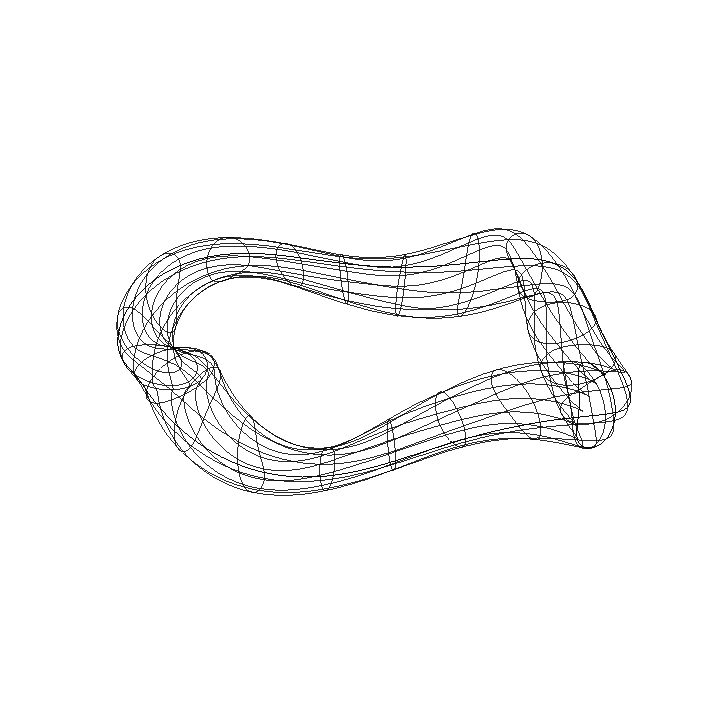
\includegraphics[width=1.18\linewidth]{title_stellarator_bw.pdf}}
    \end{column}
    \begin{column}{0.49\textwidth}
      {\fontsize{13.5}{20}\selectfont
      \mbox{From Plasma Source Physics}\par
      \mbox{to Automated Shielding Design}\par
      \mbox{in Stellarators}\par}

      \vspace{0.34cm}
      {\color{jqdark}\rule{\linewidth}{0.8pt}}

      \vspace{0.27cm}
      {\fontsize{9.5}{12}\selectfont Thaddaeus Kiker\par}
      {\fontsize{7.5}{10}\selectfont
      MIT Plasma Science and Fusion Center\par
      August 26th, 2026\par}
    \end{column}
  \end{columns}
  \note{The opening image is the reactor-scale QH VMEC boundary with its three-dimensional deformation moderated toward the toroidal mean. It retains a real stellarator field-period structure without the full-strength surface's excessive visual torsion.\notesources{Engineering illustration: \localpath{spf_prototype/talk/gen_summer_recap_figures.py}. Theme: Samuel Manchajm, Jacquenetta Beamer Theme, CC BY-SA 4.0.}}
\end{frame}}

% Intro image
{\setbeamertemplate{footline}{}
\begin{frame}[plain,noframenumbering]
  \centering
  \setlength{\fboxsep}{0pt}
  \setlength{\fboxrule}{0.65pt}
  \fbox{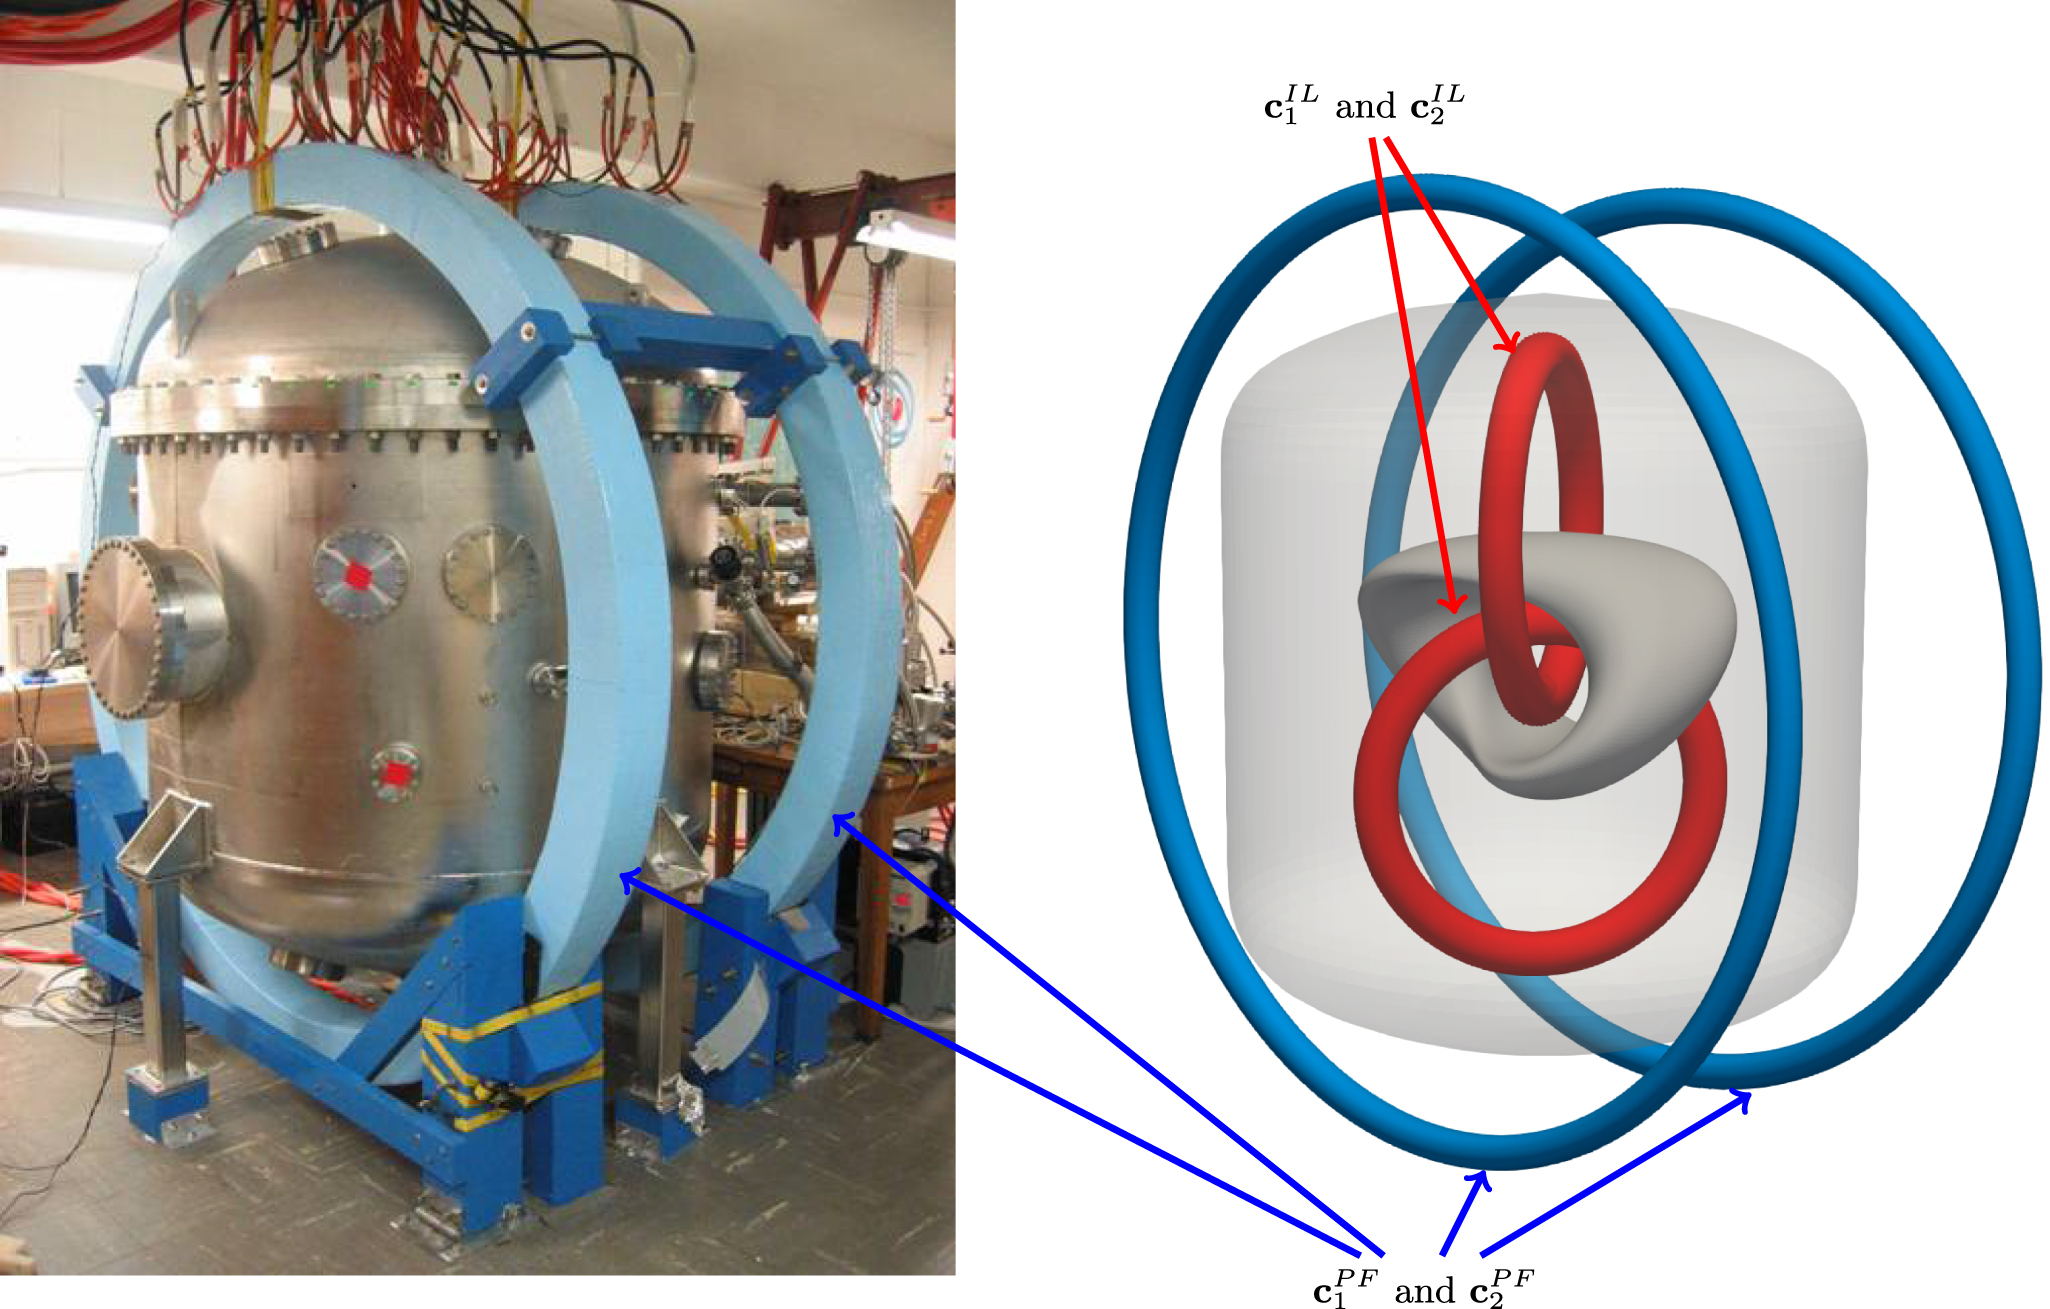
\includegraphics[height=0.90\paperheight]{intro_nfada6ddf1_hr.jpg}}
  \note{Use this image to introduce yourself and the experimental context before the technical contents slide.\notesources{User-supplied image: \localpath{/Users/tkiker/Downloads/nfada6ddf1_hr.jpg}.}}
\end{frame}}

% 2
\begin{frame}{Contents}
  \vfill
  \begin{enumerate}
    \setlength\itemsep{0.45cm}
    \item Native \texttt{StellaratorSource} in OpenMC
    \item Spin-Polarized Plasma Neutronics
    \item Automatic Reactor Shielding Optimization
  \end{enumerate}
  \vfill
\end{frame}

% 3
{\setbeamertemplate{footline}{}
\begin{frame}[plain,noframenumbering]
  \vfill
  {\fontsize{12}{14}\selectfont I\par}
  \vspace{0.38cm}
  {\fontsize{22}{27}\selectfont Native \texttt{StellaratorSource}\par in OpenMC\par}
  \vfill
\end{frame}}

% 4
\begin{frame}{Tokamaks vs. Stellarators: A Tale as Old as MCF}
  \centering
  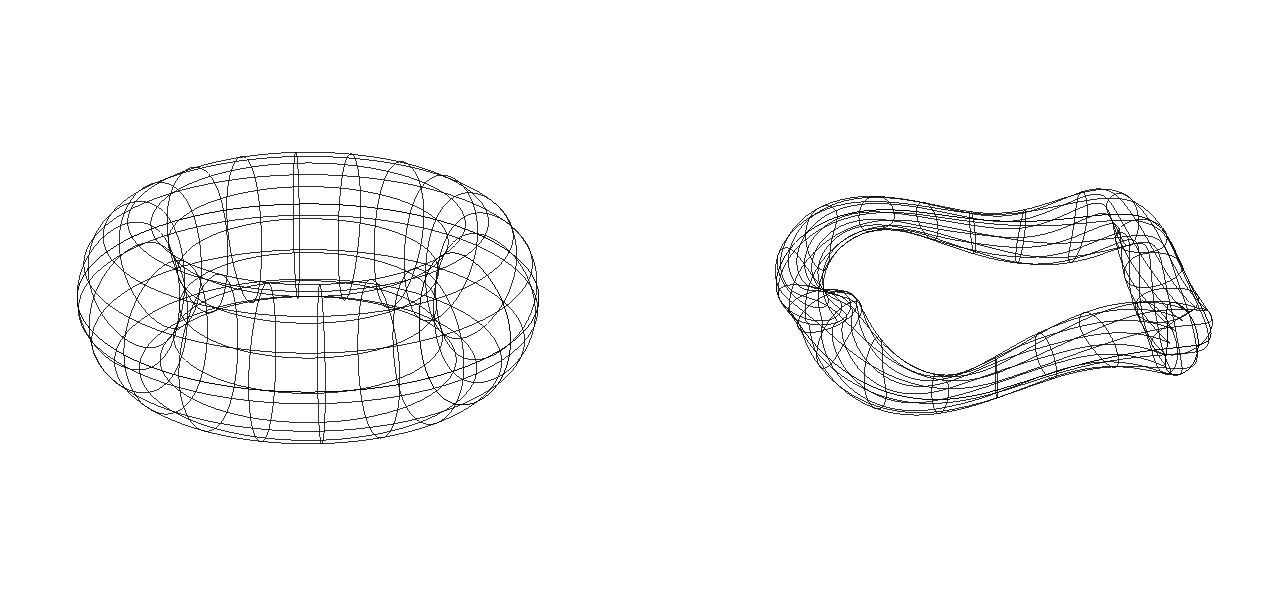
\includegraphics[width=0.88\linewidth]{tokamak_vs_stellarator_bw.pdf}

  \vspace{-0.04cm}
  \emph{One (or many) poloidal sections to rule them $\phi$ all?}
  \note{This is the source-model distinction. A tokamak admits a compact analytic surface parameterization. A general stellarator requires its equilibrium coordinates and volume element throughout the plasma. The right-hand surface is intentionally mild so the three-dimensional distinction is visible without overwhelming the comparison.\notesources{Engineering illustrations: \localpath{spf_prototype/talk/gen_summer_recap_figures.py}.}}
\end{frame}

% 4
\begin{frame}{Building a General Stellarator Source in OpenMC}
  \begin{columns}[c,onlytextwidth]
    \begin{column}{0.47\textwidth}
      \begin{center}
        {\fontsize{10.5}{13}\selectfont Peterson PR \#3999\par}
        \vspace{0.10cm}
        {\fontsize{8.5}{10.5}\selectfont Native parametric \texttt{TokamakSource}\par}
        \vspace{0.23cm}
        $\downarrow$
        \vspace{0.20cm}

        {\fontsize{10.5}{13}\selectfont \texttt{StellaratorSource}\par}
        \vspace{0.10cm}
        {\fontsize{8.5}{10.5}\selectfont VMEC geometry and local field\par}
      \end{center}
    \end{column}
    \begin{column}{0.47\textwidth}
      The OpenMC source object, XML path, and Python API remain native.

      \vspace{0.28cm}
      The analytic Miller position model is replaced by an equilibrium-supplied three-dimensional grid.

      \vspace{0.28cm}
      Each sampled birth carries the local $\Bhat$ needed by the polarized angular kernel.
    \end{column}
  \end{columns}
  \note{Dr. Ethan Peterson's PR \#3999 established the native OpenMC pattern: sample the correct joint spatial distribution, expose it through the Python/XML source API, and avoid a user-script point cloud. The stellarator extension keeps that pattern but replaces axisymmetry with a VMEC flux map.\notesources{Peterson PR note: \localpath{/Users/tkiker/Documents/Obsidian/Native parametric tokamak source PR 3999.md}. Peterson, Romano, and Dunn, On Sampling Of Parametric Tokamak Neutron Sources For Monte Carlo Radiation Transport Simulations, \localpath{/Users/tkiker/Downloads/plasma_source_sampling_paper.pdf}. Stellarator implementation: \localpath{spf_prototype/native_spf}.}}
\end{frame}

% 5
\begin{frame}{Integrating VMEC (I/II): Three-Dimensional Plasma Coordinates}
  \begin{columns}[c,onlytextwidth]
    \begin{column}{0.56\textwidth}
      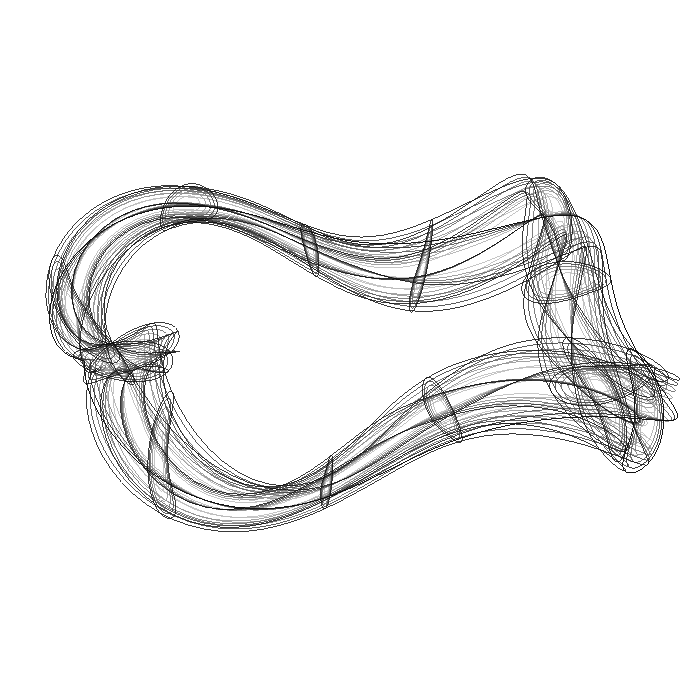
\includegraphics[width=0.90\linewidth]{vmec_coordinates_bw.pdf}
    \end{column}
    \begin{column}{0.38\textwidth}
      VMEC originated as a variational method for three-dimensional ideal-MHD equilibria.

      \vspace{0.27cm}
      Its nested flux surfaces define
      \[
        \mathbf{r}(\rho,\vartheta,\zeta)
      \]
      and the physical volume element
      \[
        \mathrm{d}V=\sqrt{g}\,
        \mathrm{d}\rho\,\mathrm{d}\vartheta\,\mathrm{d}\zeta.
      \]
    \end{column}
  \end{columns}
  \note{VMEC is the Variational Moments Equilibrium Code. The nested wireframes are five flux surfaces from the actual QH equilibrium, not a decorative torus. The source consumes the coordinate map and Jacobian; it does not solve the equilibrium inside OpenMC.\notesources{Hirshman and Whitson, Physics Of Fluids 26, 3553 (1983), Steepest-Descent Moment Method For Three-Dimensional Magnetohydrodynamic Equilibria. QH VMEC output: \localpath{spf_prototype/talk/geom/wout_qh.nc}.}}
\end{frame}

% 6
\begin{frame}{Integrating VMEC (II/II): Neutron Birth and Local $\Bhat$}
  \begin{columns}[c,onlytextwidth]
    \begin{column}{0.54\textwidth}
      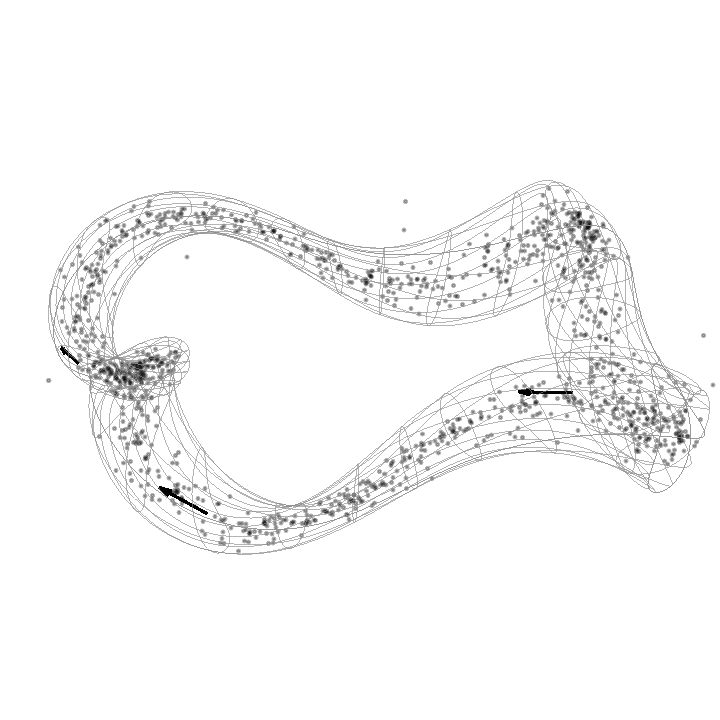
\includegraphics[width=0.86\linewidth]{source_births_bw.pdf}
    \end{column}
    \begin{column}{0.40\textwidth}
      \[
        \mathrm{d}P\propto
        S(\rho)\,\lvert\sqrt{g}\rvert\,
        \mathrm{d}\rho\,\mathrm{d}\vartheta\,\mathrm{d}\zeta
      \]
      \[
        p(\rho)\,
        p(\zeta\mid\rho)\,
        p(\vartheta\mid\rho,\zeta)
      \]
      \[
        \Bhat=\frac{\mathbf{B}}{\lvert\mathbf{B}\rvert},
        \qquad w=1
      \]
      The conditional CDF cascade is rejection free.
    \end{column}
  \end{columns}
  \note{The birth density is a profile in flux radius multiplied by the physical volume measure. The same grid supplies the local field frame. The sampler draws rho, then zeta conditional on rho, then theta conditional on both, followed by within-cell jitter and trilinear interpolation.\notesources{Algorithm and gates: \localpath{spf_prototype/native_spf/README_stellarator.md}. Python mirror: \localpath{spf_prototype/python/stellarator_source.py}.}}
\end{frame}

% 7
\begin{frame}{StellaratorSource Validation (I/II)}
  \centering
  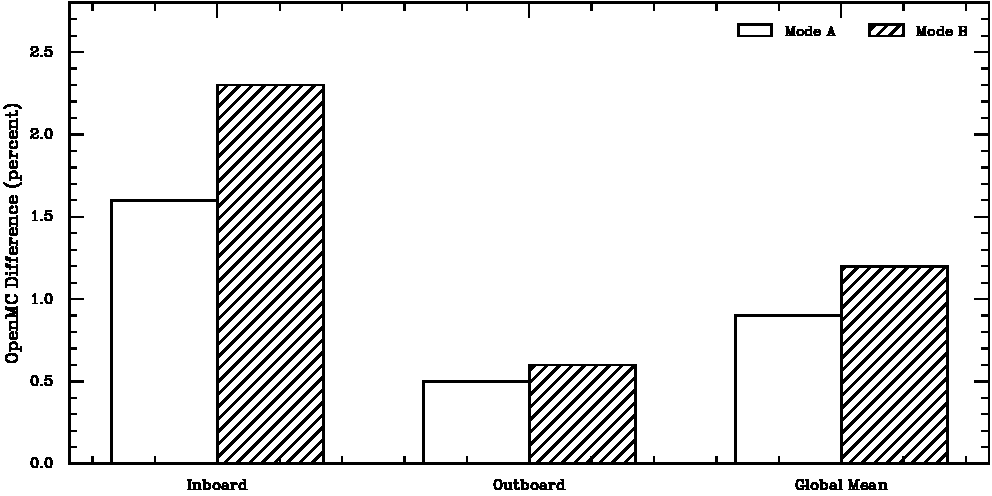
\includegraphics[width=0.62\linewidth]{transport_validation.pdf}

  \vspace{-0.12cm}
  \begin{minipage}{0.91\linewidth}
    {\fontsize{9.1}{11.0}\selectfont
    \begin{itemize}
      \item Axisymmetric free streaming: $256$-node Gauss--Legendre quadrature agrees with Schwartz's \texttt{anarrima} closed forms.
      \item Real conformal wall: an independent point--patch sum gives $0.5$--$2.3\%$ regional residuals and $0.914/0.920$ bin correlations.
    \end{itemize}
    }
  \end{minipage}
  \note{The axisymmetric oracle uses 256-node Gauss--Legendre quadrature for the free-streaming neutron-wall-loading integral. The true three-dimensional conformal-wall check is separate and uses a deterministic sum over source voxels and wall patches. The bars show percent differences, not ratios that could be mistaken for 30 percent errors.\notesources{Quadrature: \localpath{spf_prototype/python/analytic_nwl.py}. Conformal cross-check: \localpath{spf_prototype/python/conformal_freestream_xcheck.py}; frozen values: \localpath{spf_prototype/paper/data/conformal_xcheck.csv}.}}
\end{frame}

% 8
\begin{frame}{StellaratorSource Validation (II/II)}
  \centering
  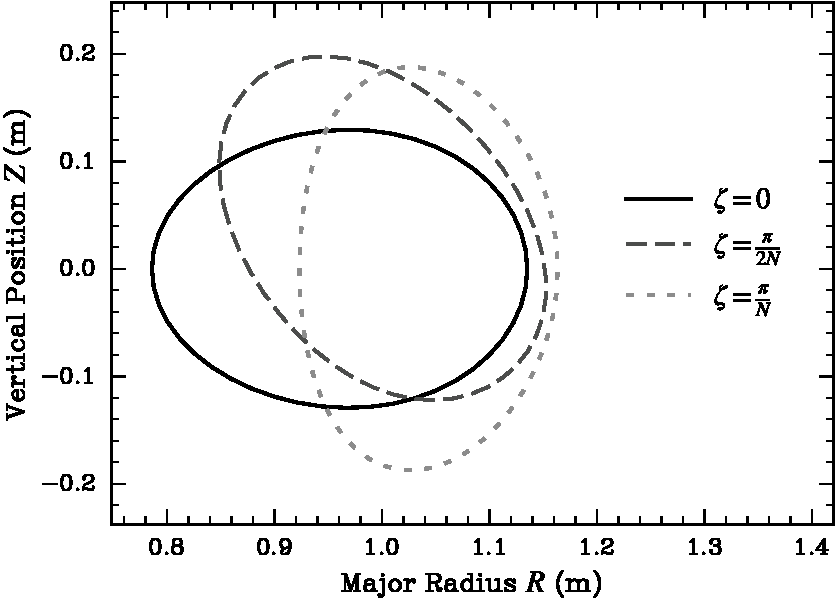
\includegraphics[height=0.54\textheight]{quasr59509_cross_sections_bw.pdf}

  \vspace{0.02cm}
  \begin{minipage}{0.88\linewidth}
    \centering
    {\fontsize{9.2}{11.0}\selectfont QUASR QA 595509}
  \end{minipage}
  \note{These are three last-closed-flux-surface sections read from the same equilibrium-derived grid consumed by the source. Device 59509 is a three-field-period quasi-axisymmetric QUASR configuration with aspect ratio about 6.7. The plot makes the non-axisymmetric rotation visible without mixing it with the transport oracle on the preceding slide. Producer-side gates separately recover VMEC volume, preserve a single-signed $\sqrt{g}$, and verify the binary round trip.\notesources{Flux map: \localpath{spf_prototype/data/quasr59509_vmec_fluxmap.npz}; plotting code: \localpath{spf_prototype/talk/gen_spf_overview_figures.py}; producer checks: \localpath{spf_prototype/python/validate_real_fluxmap.py}.}}
\end{frame}

% 9
{\setbeamertemplate{footline}{}
\begin{frame}[plain,noframenumbering]
  \vfill
  {\fontsize{12}{14}\selectfont II\par}
  \vspace{0.38cm}
  {\fontsize{22}{27}\selectfont Spin-Polarized Plasma\par Neutronics\par}
  \vfill
\end{frame}}

% 10
\begin{frame}{Overview of Spin-Polarized Fusion (I/VI): Kulsrud's Claim}
  \centering
  {\setlength{\fboxsep}{0pt}\setlength{\fboxrule}{0.55pt}%
  \fbox{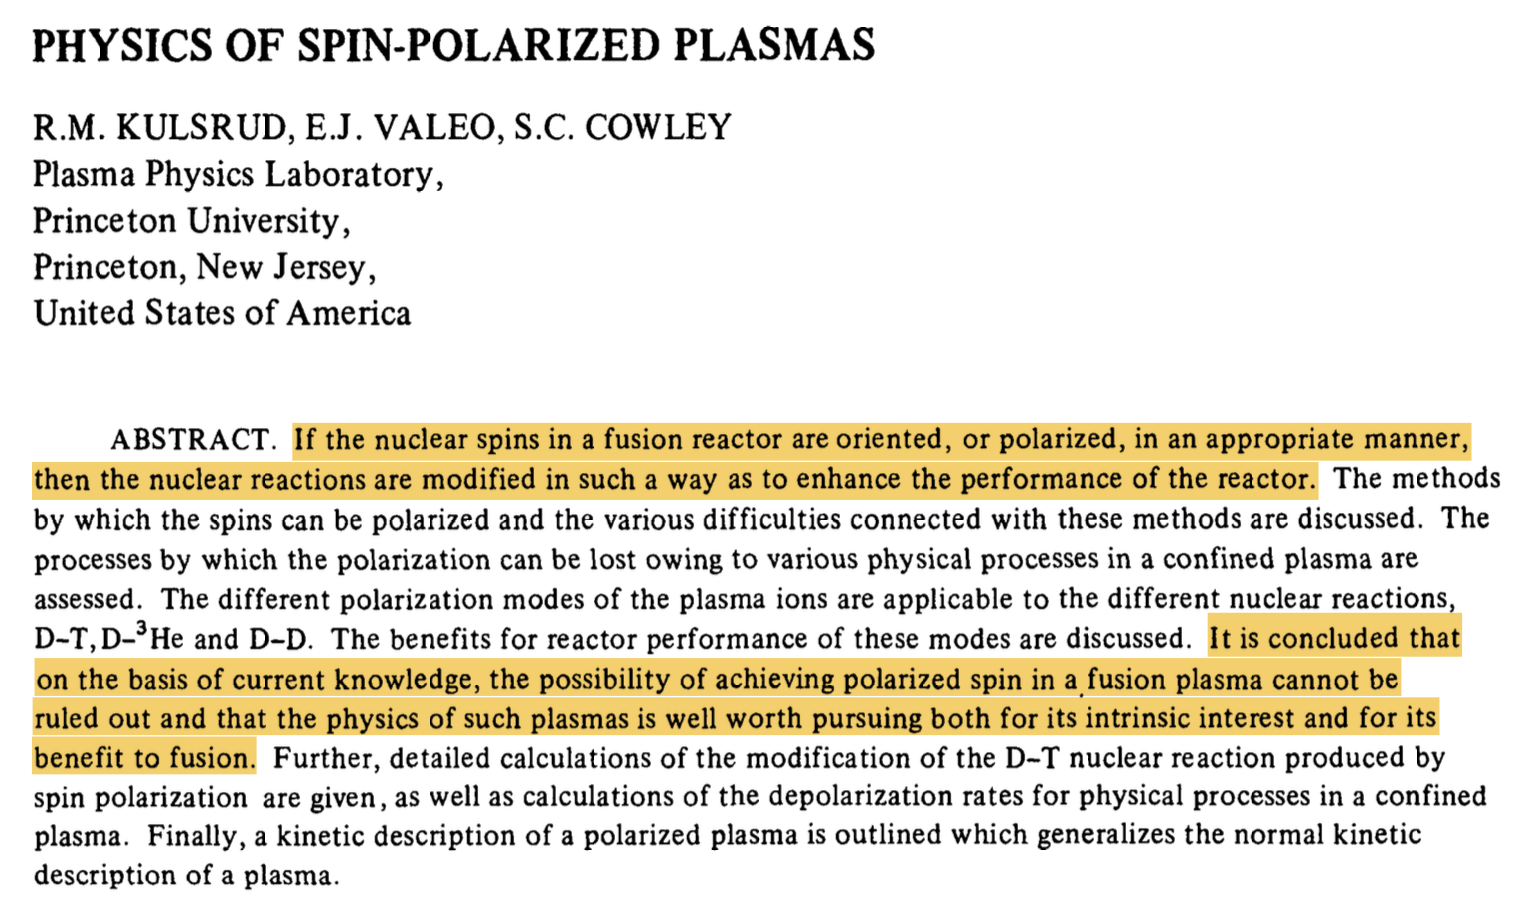
\includegraphics[width=0.71\linewidth]{kulsrud_1986_screenshot.png}}}
  \note{The screenshot is the 1986 Nuclear Fusion review by Kulsrud, Valeo, and Cowley, despite the user's source filename saying 1982. The distinct foundational 1982 paper is Kulsrud, Furth, Valeo, and Goldhaber in Physical Review Letters. The highlighted claim is the programmatic starting point: polarized fusion can improve reactor performance, and polarization survival must be established.\notesources{User-supplied screenshot: \localpath{/Users/tkiker/Desktop/Kulsrud 1982 Screenshot.png}. R. M. Kulsrud, E. J. Valeo, and S. C. Cowley, Physics of Spin-Polarized Plasmas, Nuclear Fusion 26, 1443 (1986), doi:10.1088/0029-5515/26/11/001. R. M. Kulsrud et al., Physical Review Letters 49, 1248 (1982).}}
\end{frame}

\begin{frame}{Overview of Spin-Polarized Fusion (II/VI): Nuclear-Spin States}
  \vspace{-0.22cm}
  \begin{minipage}{0.97\linewidth}
    {\fontsize{9.3}{11.2}\selectfont
    \[
      \begin{array}{rcl@{\qquad}l}
        n&=&1,2,\ldots&\text{Principal level (energy and shell size)},\\
        \ell&=&0,1,\ldots,n-1&\text{Orbital }L\text{ (orbital shell shape)},\\
        m_{\ell}&=&-\ell,\ldots,+\ell&\text{Orbital }L_z\text{ (orbital spatial orientation)},\\
        m_s&=&-\frac{1}{2},+\frac{1}{2}&\text{Intrinsic-spin projection}.
      \end{array}
    \]

    \vspace{-0.05cm}
    For a composite nucleus, angular momenta couple to total nuclear spin $I$ and its field-axis projection $m_I$:
    \[
      I_D=1,\quad m_D\in\{-1,0,+1\};
      \qquad
      I_T=\frac{1}{2},\quad m_T\in\left\{-\frac{1}{2},+\frac{1}{2}\right\}.
    \]

    \vspace{-0.04cm}
    With $d_{+},d_0,d_{-}$ and $t_{+},t_{-}$ denoting substate populations,
    \vspace{-0.24cm}
    \[
      a=d_{+}t_{+}+d_{-}t_{-},\qquad
      b=d_0t_{+}+d_0t_{-},\qquad
      c=d_{+}t_{-}+d_{-}t_{+},
      \qquad a+b+c=1.
    \]
    }
  \end{minipage}
  \note{The four textbook quantum numbers are useful orientation, but the transport model does not manipulate electronic orbitals. It uses nuclear-spin populations. Deuterium has nuclear spin one and three magnetic substates. Tritium has nuclear spin one half and two magnetic substates. The plus and minus labels on tritium are shorthand for $m_T=+1/2$ and $-1/2$, not plus and minus one. The quantities $a$, $b$, and $c$ are population sums, not coherent quantum superpositions.\notesources{State grouping and transport parameterization: \localpath{spf_prototype/paper/manuscript/spf_openmc.tex}; R. M. Kulsrud et al., Physical Review Letters 49, 1248 (1982).}}
\end{frame}

\begin{frame}{Overview of Spin-Polarized Fusion (III/VI): Spin States Along $\Bhat$}
  \centering
  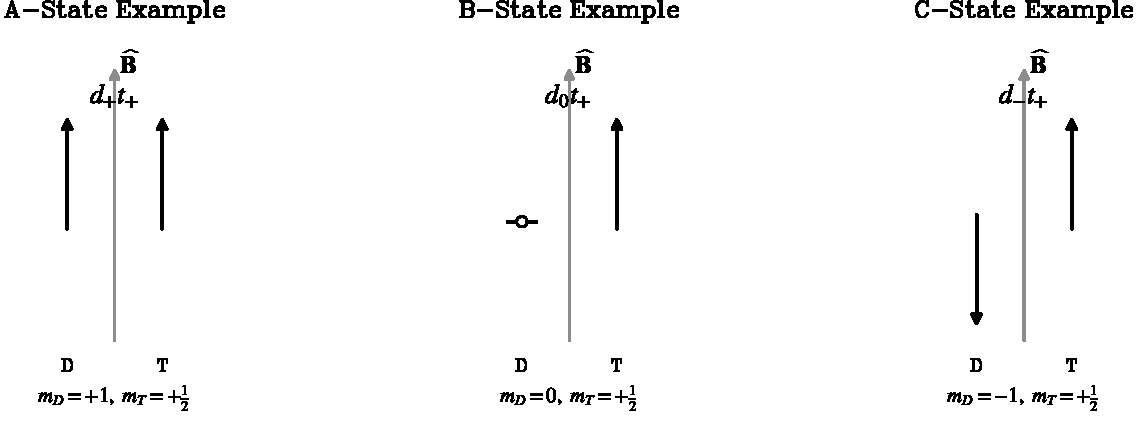
\includegraphics[width=0.91\linewidth]{spin_substates_bw.pdf}

  \vspace{0.02cm}
  {\fontsize{9.0}{10.8}\selectfont The local field defines the quantization axis for prepared spin populations; it does not create high polarization by itself.}
  \note{The A-state examples have same-sign D and T projections, either both along or both against the field. B contains the deuterium $m_D=0$ population. C has opposite-sign projections. The sketches are projection glyphs, not classical rigid dipoles: in particular, $m_D=0$ means zero projection on the field axis, not a permanently transverse classical spin. Prepared nuclei precess about the local field, which supplies the natural reference axis.\notesources{Figure: \localpath{spf_prototype/talk/gen_spf_overview_figures.py}; field-axis discussion: \localpath{spf_prototype/docs/analytic upgraded.tex}.}}
\end{frame}

\begin{frame}{Overview of Spin-Polarized Fusion (IV/VI): Emission About $\Bhat$}
  \centering
  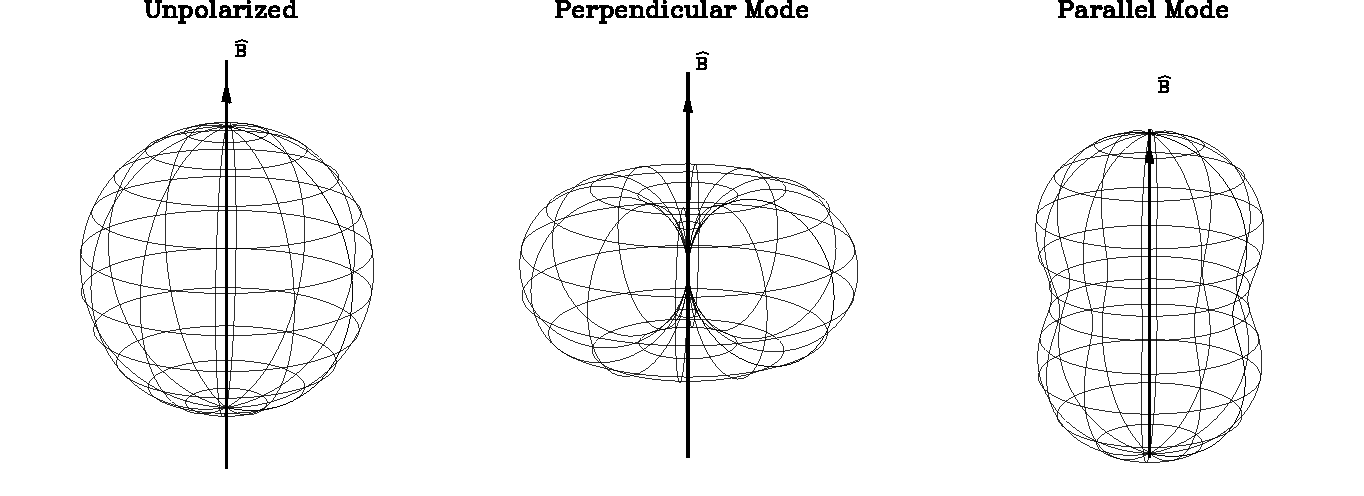
\includegraphics[width=0.95\linewidth]{spf_geometry_bw.pdf}

  \vspace{0.12cm}
  Polarizing the reacting fuel changes both the fusion yield and the neutron emission pattern relative to the local magnetic field.
  \note{The wireframes are radial plots of the normalized angular probability density. The perpendicular kernel suppresses emission along the field; the parallel kernel enhances it. The axis is the local B direction, so the same kernel can be rotated into a tokamak or stellarator field frame.\notesources{Kernel implementation: \localpath{spf_prototype/python/spf_mirror.py}. Physics derivation and references: \localpath{spf_prototype/paper/manuscript/spf_openmc.tex}.}}
\end{frame}

\begin{frame}{Overview of Spin-Polarized Fusion (V/VI): Alpha Heating}
  \centering
  \vfill
  \begin{minipage}{0.90\linewidth}
    {\fontsize{9.7}{11.8}\selectfont
    A-State Reactivity: Same-sign D--T spin projections give
    \[
      \frac{\sigma_A}{\sigma_0}=\frac{3}{2},
      \qquad
      \frac{\mathrm{d}\sigma_A}{\mathrm{d}\Omega}\propto\sin^2\theta,
      \qquad \cos\theta=\Bhat\cdot\uhat.
    \]

    \vspace{0.14cm}
    Alpha Self-Heating: More reactions produce more $3.5\ \mathrm{MeV}$ alpha particles. Their heating raises the plasma temperature, so burn feedback can increase fusion power by more than the $50\%$ cross-section gain alone.
    }
  \end{minipage}
  \vfill
  \note{The enhanced state is A: the deuteron and triton projections have the same sign. Both the neutron and alpha angular distributions inherit the perpendicular $\sin^2\theta$ shape because the two products are born back to back. The standard claim that fusion power can increase by more than 50 percent comes from nonlinear alpha self-heating: more reactions create more 3.5 MeV alphas, which heat the fuel and increase reactivity. It is not justified by saying perpendicular birth makes the alpha Larmor radius smaller; $r_{L\alpha}$ actually grows with $v_\perp$. That orbit question belongs to fast-ion transport and is treated explicitly in the backup slide.\notesources{Heidbrink et al., Frontiers in Physics 12, 1355212 (2024), doi:10.3389/fphy.2024.1355212; Kulsrud et al., Physical Review Letters 49, 1248 (1982).}}
\end{frame}

\begin{frame}{Overview of Spin-Polarized Fusion (VI/VI): Polarization Lifetime}
  \centering
  {\setlength{\fboxsep}{0pt}\setlength{\fboxrule}{0.55pt}%
  \fbox{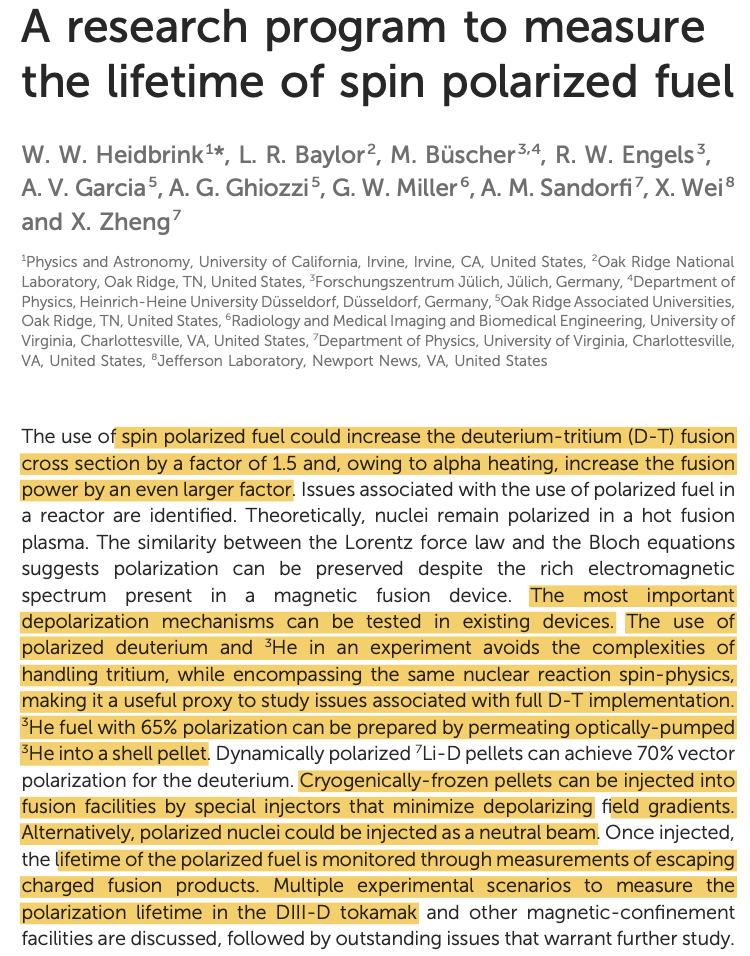
\includegraphics[height=0.73\textheight]{spf_research_program_screenshot.png}}}
  \note{This slide is intentionally an invitation rather than a detour. Tell the audience that polarization preparation, depolarization, and the DIII-D lifetime program are active experimental questions, then point them to the backup slides if they want the deeper discussion. The screenshot is the 2024 research-program paper.\notesources{User-supplied screenshot: \localpath{/Users/tkiker/Desktop/spf research program screenshot.png}. Heidbrink et al., Frontiers in Physics 12, 1355212 (2024), doi:10.3389/fphy.2024.1355212.}}
\end{frame}

% 11
\begin{frame}{Spin-Polarized Fusion Changes Rate and Emission Angle}
  \[
    \frac{\mathrm{d}\sigma}{\mathrm{d}\Omega}
    =\frac{\sigma_0}{2\pi}
    \left[
      \frac{3}{4}a\sin^2\theta
      +\left(\frac{2}{3}b+\frac{1}{3}c\right)
       \left(\frac{1}{4}+\frac{3}{4}\cos^2\theta\right)
    \right],
    \qquad \cos\theta=\Bhat\cdot\uhat
  \]

  \vspace{0.20cm}
  \centering
  \begin{tabular}{lccc}
    \toprule
    Mode & $(a,b,c)$ & Rate / Unpolarized Rate & Emission Relative to $\Bhat$ \\
    \midrule
    Unpolarized & $\left(\frac{1}{3},\frac{1}{3},\frac{1}{3}\right)$ & $1$ & Isotropic \\
    A & $(1,0,0)$ & $\frac{3}{2}$ & Perpendicular \\
    B & $(0,1,0)$ & $1$ & Parallel \\
    C & $(0,0,1)$ & $\frac{1}{2}$ & Parallel \\
    \bottomrule
  \end{tabular}
  \note{The rate and angle cannot be separated in an engineering comparison. B and C share the same normalized angular kernel but have different reaction rates. A increases the rate while steering perpendicular to B.\notesources{Frozen model statement: \localpath{spf_prototype/paper/manuscript/spf_openmc.tex}.}}
\end{frame}

\begin{frame}{Prior Spin-Polarized Fusion Neutronics}
  \centering
  \begin{tabular}{@{}c@{\hspace{0.34cm}}c@{}}
    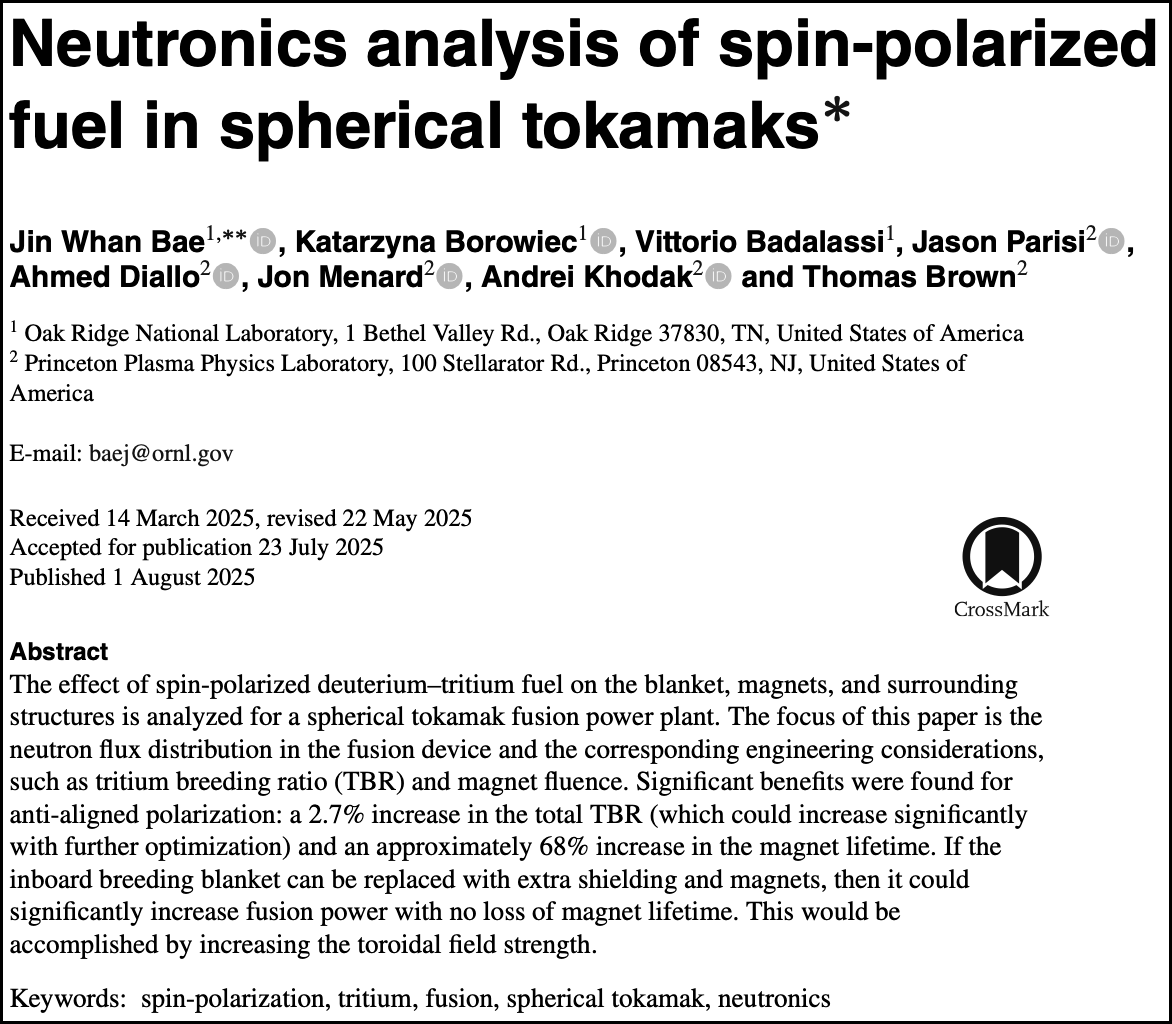
\includegraphics[height=0.57\textheight]{bae_screenshot_bw.png} &
    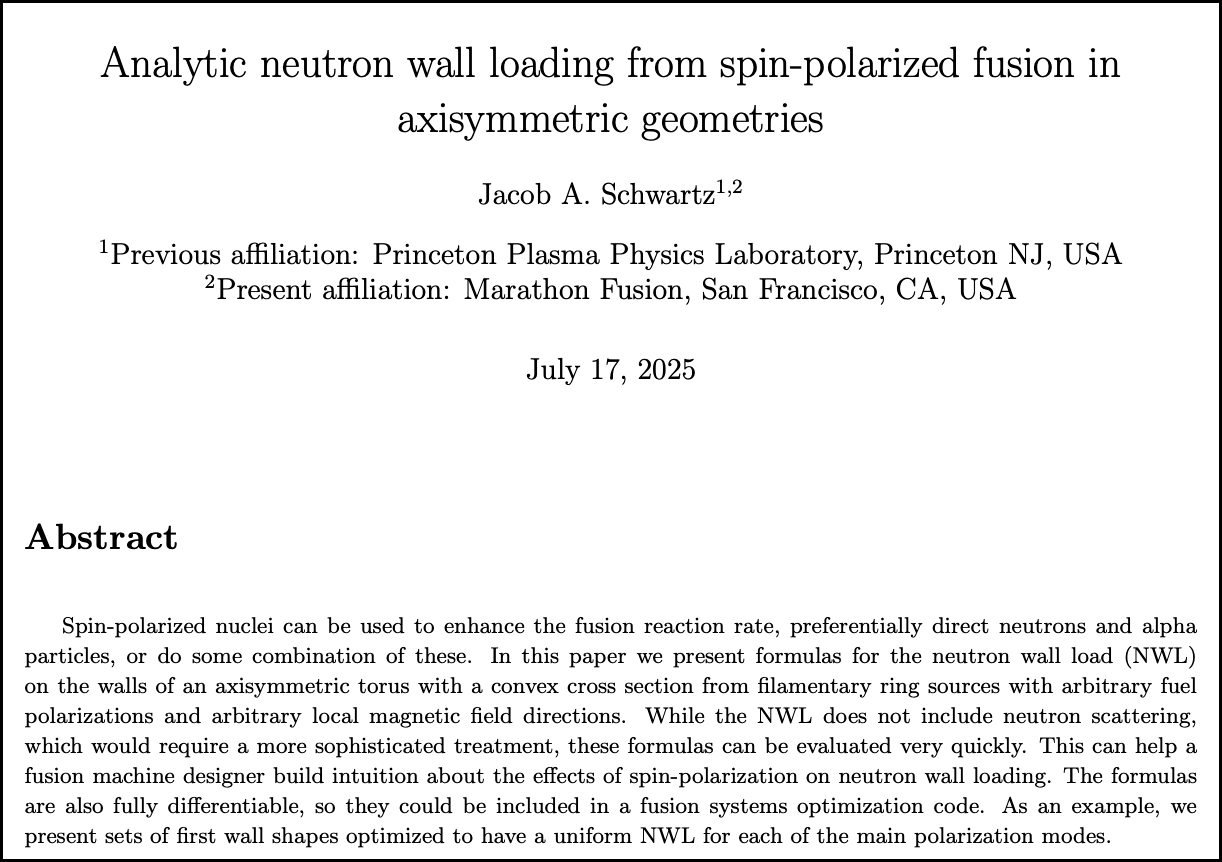
\includegraphics[height=0.57\textheight]{schwartz_screenshot_bw.png}
  \end{tabular}
  \note{Bae et al. provide the closest Monte Carlo precedent: a precomputed polarized source bank in a spherical-tokamak OpenMC model. Schwartz provides the independent analytic free-streaming neutron-wall-loading benchmark for axisymmetric geometries.\notesources{User-selected screenshots derived from Bae et al., Nuclear Fusion 65, 086051 (2025), and Schwartz, arXiv:2507.11758 (2025). Repository copies: \localpath{spf_prototype/talk/figs/paper_screenshots}.}}
\end{frame}

% 12
\begin{frame}{Proposed StellaratorSource Interface for OpenMC}
  \begin{center}
  \begin{minipage}{0.76\textwidth}
    \begin{minipage}[c]{0.48\linewidth}
      {\ttfamily\fontsize{7.3}{9.2}\selectfont
      src = openmc.StellaratorSource(\par
      \hspace{0.45cm}fluxmap="qh\_fluxmap",\par
      \hspace{0.45cm}polarization=(a, b, c),\par
      \hspace{0.45cm}field\_model="fluxmap",\par
      \hspace{0.45cm}energy=openmc.stats.Discrete(\par
      \hspace{0.90cm}[14.06e6], [1.0]),\par
      \hspace{0.45cm}strength=1.0)\par}
    \end{minipage}
    \hfill
    \begin{minipage}[c]{0.45\linewidth}
      \raggedright
      Compact Runtime Format

      \hspace{0.32cm}\texttt{.meta + .bin}

      \vspace{0.26cm}
      Python and XML use the existing source API

      \vspace{0.26cm}
      Isotropic behavior remains the default

      \vspace{0.26cm}
      Equilibrium conversion stays outside transport
    \end{minipage}
  \end{minipage}
  \end{center}
  \note{The source is reusable because the OpenMC runtime sees a compact equilibrium-derived map rather than a device-specific Python point cloud. The native snapshot is still based on the PR \#3999 branch and requires upstream integration work before release.\notesources{API and file format: \localpath{spf_prototype/native_spf/README_stellarator.md}; integration status: \localpath{spf_prototype/native_spf/openmc_integration/README.md}.}}
\end{frame}

% 13
\begin{frame}{One Kernel Supports Tokamak and Stellarator Sources}
  \begin{columns}[T,onlytextwidth]
    \begin{column}{0.46\textwidth}
      \centering {\fontsize{10}{12}\selectfont Tokamak\par}
      \slideline
      \begin{minipage}[t][2.25cm][t]{0.96\linewidth}
      {\ttfamily\fontsize{7.1}{9}\selectfont
      openmc.TokamakSource(\par
      \hspace{0.35cm}major\_radius=...,\par
      \hspace{0.35cm}minor\_radius=...,\par
      \hspace{0.35cm}polarization=(a,b,c),\par
      \hspace{0.35cm}field\_model="pitched")\par}
      \end{minipage}
      \par\raggedright Miller birth-position sampler extended with toroidal or $q$-profile-pitched $\Bhat$ and SPF emission.
    \end{column}
    \begin{column}{0.46\textwidth}
      \centering {\fontsize{10}{12}\selectfont Stellarator\par}
      \slideline
      \begin{minipage}[t][2.25cm][t]{0.96\linewidth}
      {\ttfamily\fontsize{7.1}{9}\selectfont
      openmc.StellaratorSource(\par
      \hspace{0.35cm}fluxmap="qh\_fluxmap",\par
      \hspace{0.35cm}polarization=(a,b,c),\par
      \hspace{0.35cm}field\_model="fluxmap")\par}
      \end{minipage}
      \par\raggedright VMEC position model with the gridded local magnetic field.
    \end{column}
  \end{columns}

  \vspace{0.36cm}
  \centering
  The angular mixture, inverse CDF, and three-dimensional rotation are shared.
  \note{The tokamak path extends the PR \#3999 Miller birth-position sampler with toroidal or q-profile-pitched local field directions and SPF emission. The stellarator path replaces the spatial and local-field model with the VMEC flux map while reusing the angular mixture, inverse-CDF sampler, and three-dimensional rotation. This is the integrated patch snapshot, not ordinary OpenMC develop.\notesources{Tokamak patch and integration status: \localpath{spf_prototype/native_spf/README_apply.md}; stellarator source: \localpath{spf_prototype/native_spf/README_stellarator.md}.}}
\end{frame}

% 14
\begin{frame}{SPF Kernel Validation (I/III)}
  \centering
  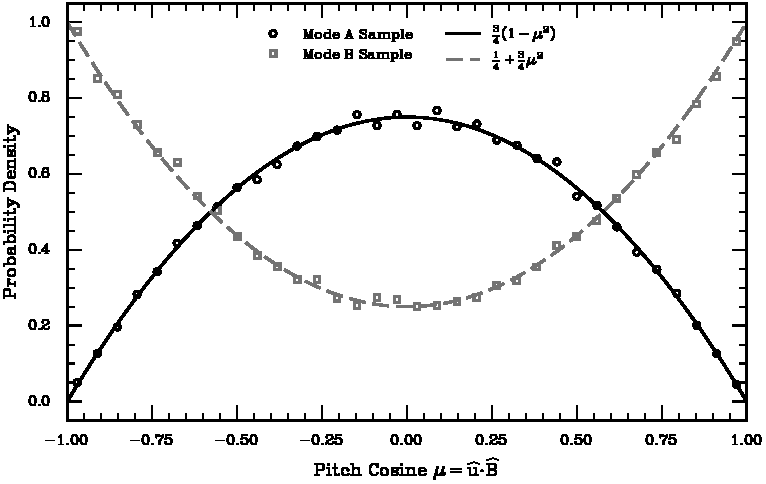
\includegraphics[width=0.67\linewidth]{sampler_validation.pdf}
  \note{Markers are Monte Carlo direction samples; lines are analytic probability densities. This isolates the angular sampler before geometry and transport are introduced.\notesources{Statistical tests: \localpath{spf_prototype/tests/test_sampler_stats.py}; independent mirror: \localpath{spf_prototype/python/spf_mirror.py}.}}
\end{frame}

% 15
\begin{frame}{SPF Kernel Validation (II/III)}
  \centering
  \begin{columns}[c,totalwidth=0.90\textwidth]
    \begin{column}{0.51\textwidth}
      \[
        G(\mathbf{w})=
        \int_{V_p}
        \frac{S(\mathbf{r})\,f(\uhat\cdot\Bhat)}
        {4\pi\lVert\mathbf{w}-\mathbf{r}\rVert^2}
        \,\mathrm{d}V
      \]

      \vspace{0.10cm}
      \centering
      OpenMC $\longleftrightarrow$ $256$-node quadrature

      \vspace{0.14cm}
      Quadrature $\longleftrightarrow$ \texttt{anarrima}
    \end{column}
    \begin{column}{0.39\textwidth}
      {\fontsize{8.1}{9.9}\selectfont
      \begin{tabular}{lrr}
        \toprule
        A Mode & Inboard & Outboard \\
        \midrule
        Schwartz text & $+43\%$ & $-22\%$ \\
        Quadrature & $+40.6\%$ & $-21.2\%$ \\
        OpenMC & $+39.2\%$ & $-21.0\%$ \\
        \bottomrule
      \end{tabular}}

      \vspace{0.28cm}
      Convex, axisymmetric, free-streaming limit.
    \end{column}
  \end{columns}
  \note{The Gaussian quadrature result and the anarrima closed form agree to numerical precision. Schwartz's paper text reports rounded values; the executable reference gives 40.6 and -21.2 percent. OpenMC reproduces the same pattern within transport and geometry approximations.\notesources{Analytic result: \localpath{spf_prototype/docs/notes/results/RESULTS_tier2a.md}; OpenMC result: \localpath{spf_prototype/docs/notes/results/RESULTS_tier2b.md}; quadrature implementation: \localpath{spf_prototype/python/analytic_nwl.py}.}}
\end{frame}

% 16
\begin{frame}{SPF Kernel Validation (III/III)}
  \centering
  \begin{minipage}{0.84\linewidth}
    {\fontsize{9.35}{11.4}\selectfont
    Schwartz (2025): in the fully polarized A state of an aspect-ratio-two box torus, the $\sin^2\theta$ kernel changes inboard and outboard NWL by $+43\%$ and $-22\%$; quadrature and OpenMC recover both.

    \vspace{0.46cm}
    Bae et al. (2025): in an ARC-class FLiBe model, parallel emission raises TBR by $2.7\%$ and lowers inboard magnet flux by $40\%$; the present model recovers both trends.
    }
  \end{minipage}
  \note{The Schwartz comparison checks the free-streaming wall-load kernel for the A mode, whose emission is perpendicular to the local toroidal magnetic field. The Bae comparison checks two full-transport trends: center-stack relief and higher TBR under parallel emission. Our ARC-class FLiBe model gives smaller magnitudes because its blanket and geometry differ.\notesources{Schwartz recovery: \localpath{spf_prototype/docs/notes/results/RESULTS_tier2b.md}. Bae comparison: \localpath{spf_prototype/docs/reference/PRIOR_WORK_BAE2025.md}; independent FLiBe results: \localpath{spf_prototype/docs/notes/results/RESULTS_tier5.md} and \localpath{spf_prototype/docs/notes/results/RESULTS_tier6.md}.}}
\end{frame}

% 17
\begin{frame}{SPF Effects (I/II): $R$ and NWL Coupling}
  \begin{columns}[c,onlytextwidth]
    \begin{column}{0.70\textwidth}
      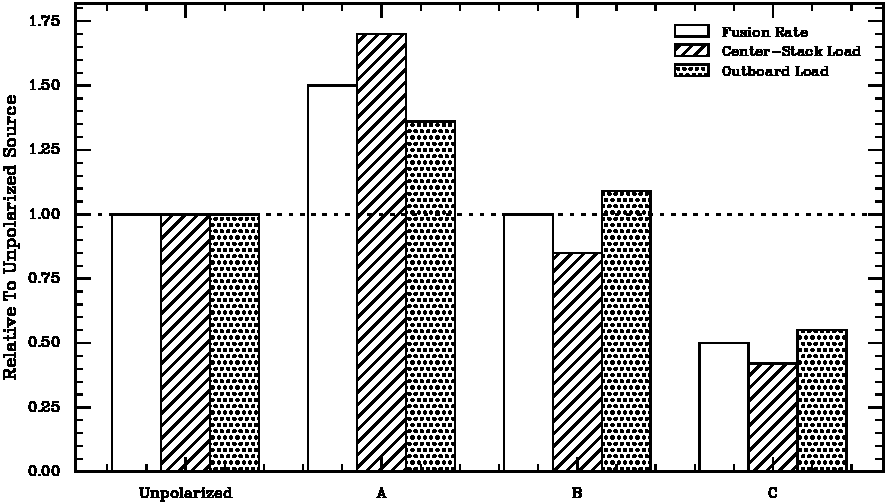
\includegraphics[width=\linewidth]{rate_steering.pdf}
    \end{column}
    \begin{column}{0.25\textwidth}
      Mode A increases the reaction rate and compounds center-stack loading.

      \vspace{0.28cm}
      Mode B changes direction without a rate increase.

      \vspace{0.28cm}
      Mode C uses the B kernel at half the unpolarized rate.
    \end{column}
  \end{columns}
  \note{This is the axisymmetric engineering control case. Directional steering remains legible because the center stack and outboard wall have simple geometric relations to the local field.\notesources{Frozen result table: \localpath{spf_prototype/paper/data/rate_steering.csv}.}}
\end{frame}

% 18
\begin{frame}{SPF Effects (II/II): Poor Peaking Reduction by Geometry}
  \centering
  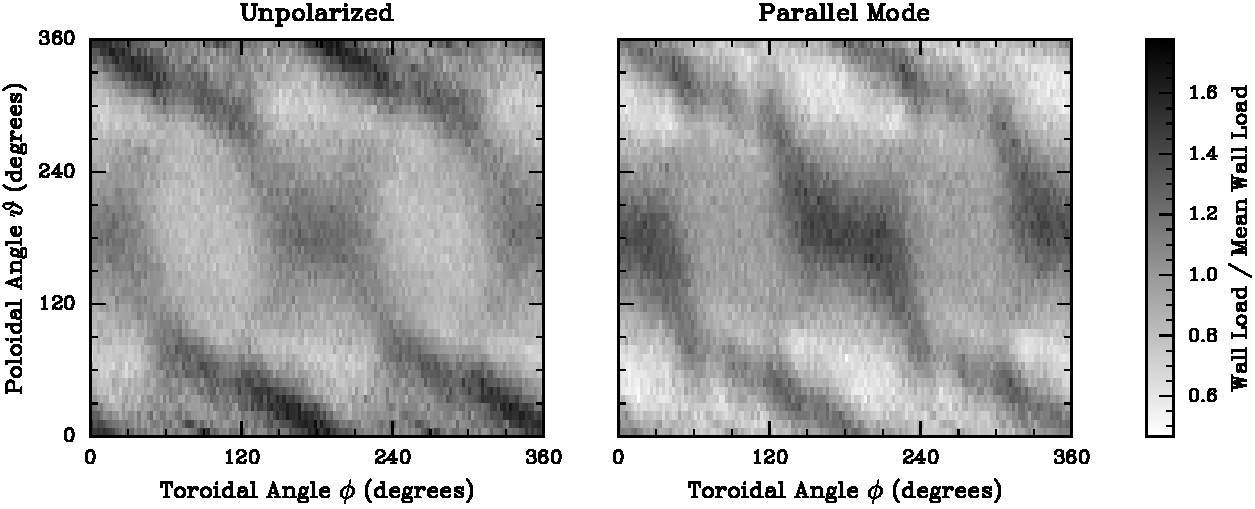
\includegraphics[width=0.78\linewidth]{conformal_map.pdf}

  \vspace{0.18cm}
  \begin{minipage}{0.89\linewidth}
    {\fontsize{9.1}{11.0}\selectfont
    Across fifteen usable QUASR equilibria, the peaking reduction has a $4.34\%$ median, a $1.24\%$--$5.67\%$ interquartile range, and a $16.05\%$ maximum.}
  \end{minipage}
  \note{The map is device 886079, the largest response in the ensemble. The statistics come from fifteen distinct QUASR equilibria, each with the same conformal wall offset of 0.30 times its minor radius. These are not fifteen wall-offset choices for one machine. Thirty VMEC attempts produced twenty-two converged equilibria and fifteen usable conformal maps; aspect ratios span 3.3 to 24 and the set is mostly QA.\notesources{Map: \localpath{spf_prototype/paper/data/conformal_maps/quasr886079_conformalmap.npz}; ensemble: \localpath{spf_prototype/paper/data/predictor_n15.csv}; pipeline notes: \localpath{spf_prototype/talk/spf_results_annotated.tex}.}}
\end{frame}

% 19
{\setbeamertemplate{footline}{}
\begin{frame}[plain,noframenumbering]
  \vfill
  {\fontsize{12}{14}\selectfont III\par}
  \vspace{0.38cm}
  {\fontsize{22}{27}\selectfont Automatic Reactor Shielding\par Optimization\par}
  \vfill
\end{frame}}

% 20
\begin{frame}{Nonuniform Shielding in Stellarator Design}
  \centering
  \begin{tabular}{@{}c@{\hspace{0.40cm}}c@{}}
    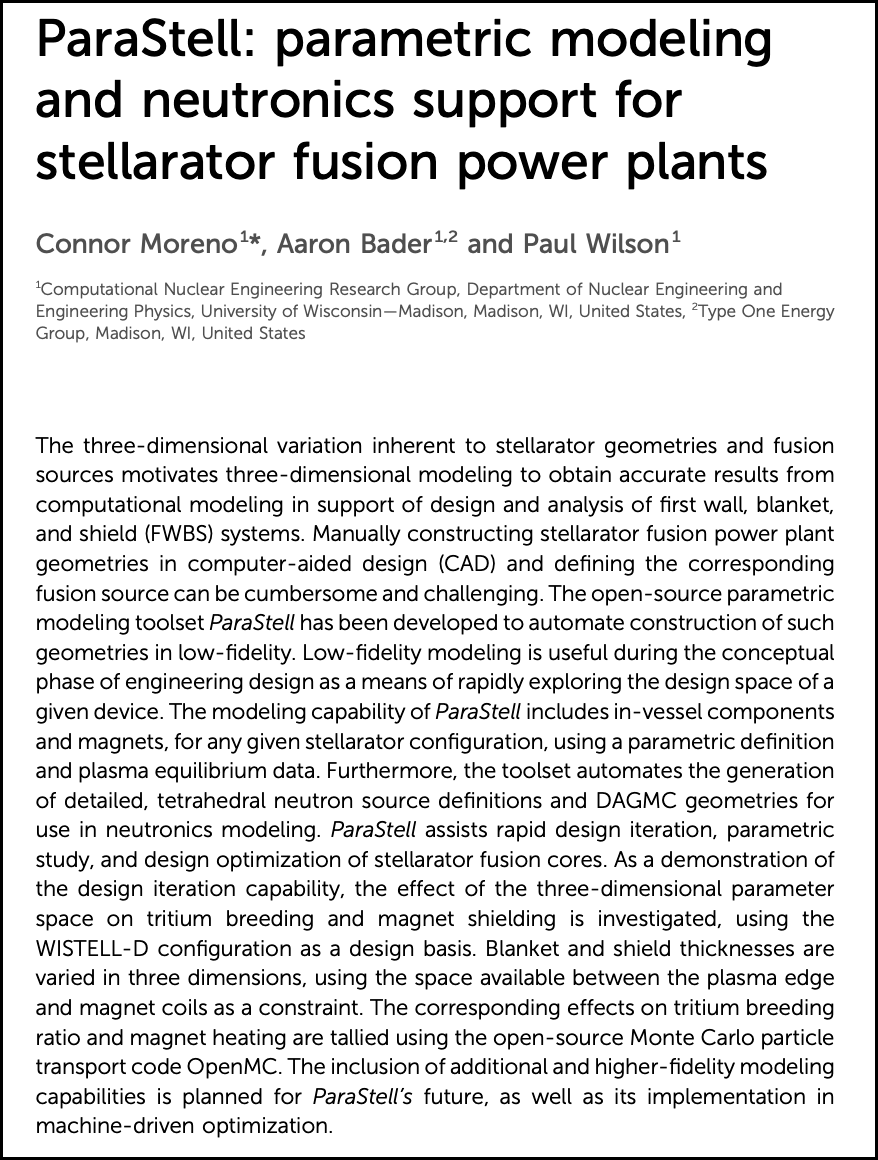
\includegraphics[height=0.61\textheight]{parastell_screenshot_bw.png} &
    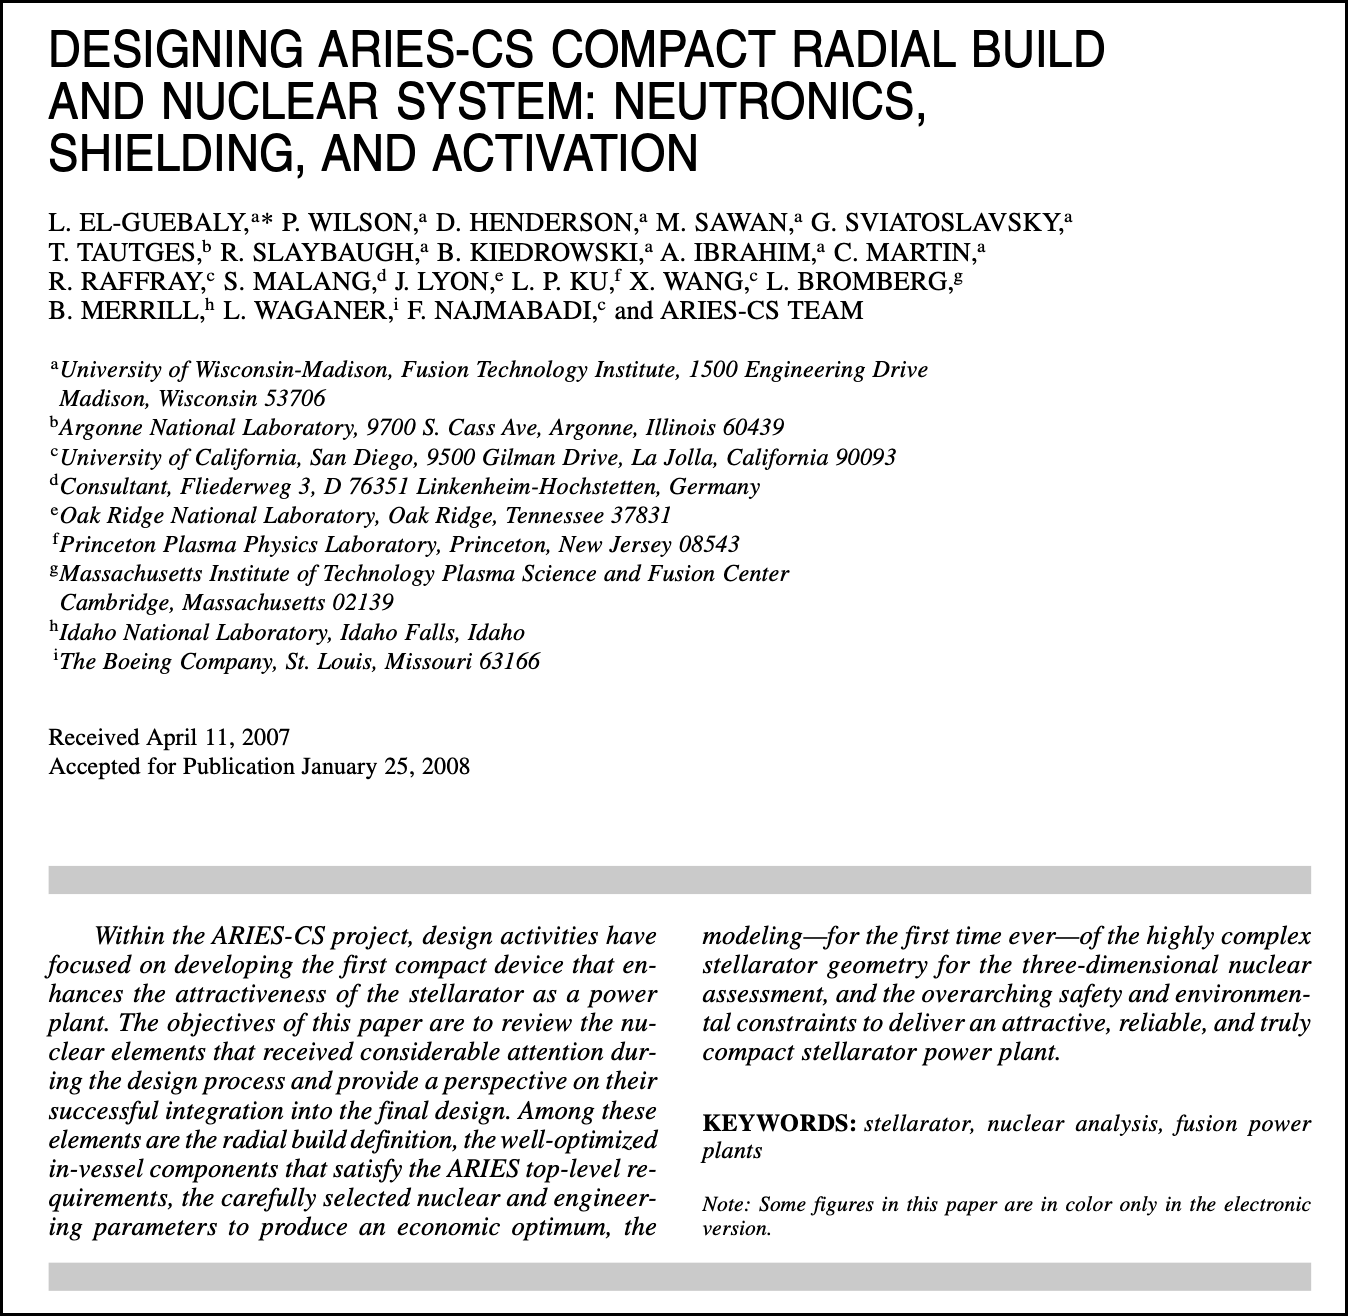
\includegraphics[height=0.61\textheight]{aries_cs_screenshot_bw.png}
  \end{tabular}
  \note{ARIES-CS established the engineering value of locally tailored blanket and shield builds in tight stellarator regions. ParaStell automated three-dimensional blanket and shield geometry generation and explicitly identified machine-driven optimization as future work.\notesources{User-selected screenshots derived from Moreno et al., Frontiers in Nuclear Engineering 3, 1384788 (2024), and El-Guebaly et al., Fusion Science and Technology 54, 747--770 (2008). Repository copies: \localpath{spf_prototype/talk/figs/paper_screenshots}.}}
\end{frame}

% 21
\begin{frame}{Parameterizing Nonuniform Blanket and Shield Thickness}
  \centering
  \begin{columns}[c,totalwidth=0.86\textwidth]
    \begin{column}{0.40\textwidth}
      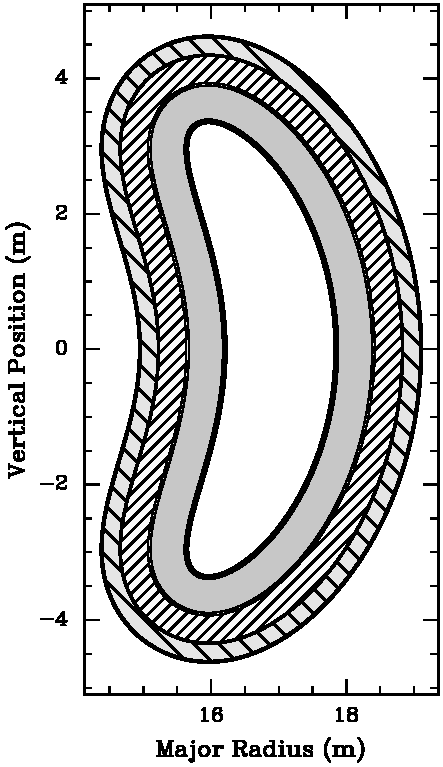
\includegraphics[height=0.69\textheight]{radial_build_bw.pdf}
    \end{column}
    \begin{column}{0.46\textwidth}
      \[
        t_{\mathrm{br}}=t_{\mathrm{br}}(\vartheta,\phi),
        \qquad
        t_{\mathrm{sh}}=t_{\mathrm{sh}}(\vartheta,\phi)
      \]

      \vspace{0.10cm}
      A design field changes the complete coil-response vector, TBR, shield mass, and maximum build.

      \vspace{0.28cm}
      The question is where material changes improve the limiting response without creating a new limit elsewhere.
    \end{column}
  \end{columns}
  \note{This is the Step-1 QH radial build: first wall, Be, FLiBe, back wall, WC shield, gap, vacuum vessel, and thermal shield. The figure deliberately omits a tiny legend; the layer identities and dimensions belong in the teaching guide and discussion.\notesources{Build definition: \localpath{spf_prototype/shield_opt/plasma_geometry.py}; geometry builder: \localpath{spf_prototype/shield_opt/patch_worth/build_step1.py}.}}
\end{frame}

% 21
\begin{frame}[t]{\mbox{Searching for a Cheap Alternative to Neutronics (I/IV)}}
  \centering
  \vfill
  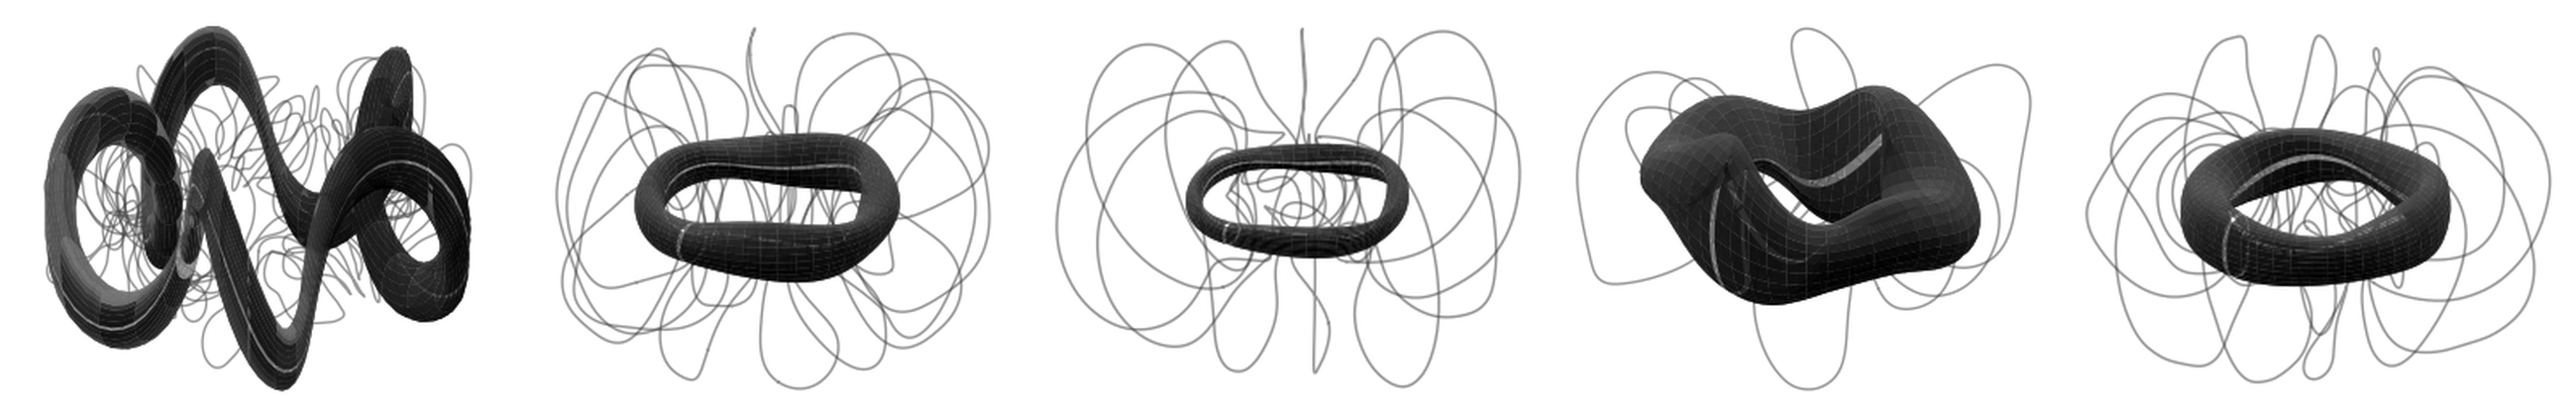
\includegraphics[width=0.98\linewidth]{config_montage_bw.png}

  \vspace{0.17cm}
  {\fontsize{8.2}{10}\selectfont
  QUASR 1960314 \hfill QUASR 59509 \hfill QUASR 803097 \hfill QUASR 886079 \hfill QUASR 932746}
  \vfill
  \note{The cheap-predictor work began with catalogue breadth, then moved to reactor-scale anchors whose plasma-to-coil spacing was suitable for shielding design. The five images are actual solved configurations, not schematic shapes.\notesources{Device renders: \localpath{spf_prototype/figs/vmec_devices}; predictor data: \localpath{spf_prototype/paper/data/predictor_n15.csv}; reactor-scale QH and QA assets: \localpath{spf_prototype/talk/geom}.}}
\end{frame}

% 22
\begin{frame}[t]{\mbox{Searching for a Cheap Alternative to Neutronics (II/IV)}}
  \centering
  \vfill
  \begin{minipage}{0.84\textwidth}
    \begin{minipage}[t]{0.46\linewidth}
      \centering
      {\fontsize{9.2}{11.0}\selectfont Geometric Wall-Load Headroom\par}
      \slideline
      \begin{minipage}[t][0.98cm][c]{\linewidth}
        \centering
        $\displaystyle
          \mathrm{PF}_{\mathrm{geo}}=
          \frac{\max_{\mathbf{w}}G(\mathbf{w})}{\langle G\rangle_A}$
      \end{minipage}
      \begin{minipage}[t][1.12cm][c]{\linewidth}
        \centering
        {\fontsize{8.0}{9.6}\selectfont
        $\displaystyle G(\mathbf{w})=\sum_v
          \frac{\lvert\sqrt{g}_v\rvert}
          {\lVert\mathbf{w}-\mathbf{r}_v\rVert^2}$}
      \end{minipage}
      \begin{minipage}[t][0.86cm][t]{0.94\linewidth}
        \raggedright Inverse-square geometry estimates wall-load headroom.
      \end{minipage}
    \end{minipage}
    \hfill
    \begin{minipage}[t]{0.46\linewidth}
      \centering
      {\fontsize{9.2}{11.0}\selectfont Effective Three-Dimensional Shaping\par}
      \slideline
      \begin{minipage}[t][0.98cm][c]{\linewidth}
        \centering
        $\displaystyle
          \varepsilon_{\mathrm{eff}}=
          \frac{\max_{\phi}\sqrt{\delta R^2+\delta Z^2}}
          {\min_{\phi}\lvert\Delta_0\rvert}$
      \end{minipage}
      \begin{minipage}[t][1.12cm][c]{\linewidth}
        \mbox{}
      \end{minipage}
      \begin{minipage}[t][0.86cm][t]{0.94\linewidth}
        \raggedright Three-dimensional excursion is normalized by the minimum source--wall standoff.
      \end{minipage}
    \end{minipage}
  \end{minipage}
  \vfill
  \note{PFgeo asks whether inverse-square geometry alone predicts peaking headroom. Epsilon effective compares intrinsic three-dimensional excursion with the minimum source-to-wall standoff and identifies when a low-order shaping approximation should fail.\notesources{Definitions and audits: \localpath{spf_prototype/talk/QA_RESEARCH.md}; predictor implementation: \localpath{spf_prototype/python/predictor_test.py}.}}
\end{frame}

% 23
\begin{frame}[t]{\mbox{Searching for a Cheap Alternative to Neutronics (III/IV)}}
  \centering
  \vfill
  \begin{minipage}{0.84\textwidth}
    \begin{minipage}[t]{0.46\linewidth}
      \centering
      {\fontsize{9.2}{11.0}\selectfont Nematic Shape Coherence\par}
      \slideline
      \begin{minipage}[t][1.48cm][c]{\linewidth}
        \centering
        $\displaystyle Q=\left\lvert\left\langle e^{2i\psi}\right\rangle\right\rvert$
      \end{minipage}
      \begin{minipage}[t][0.86cm][t]{0.94\linewidth}
        \raggedright Wall-normal field angles share a preferred axis.
      \end{minipage}
    \end{minipage}
    \hfill
    \begin{minipage}[t]{0.46\linewidth}
      \centering
      {\fontsize{9.2}{11.0}\selectfont Winding-Pack Clearance\par}
      \slideline
      \begin{minipage}[t][1.48cm][c]{\linewidth}
        \centering
        {\fontsize{8.4}{10.1}\selectfont
        $\displaystyle c(\vartheta,\phi)=\min_{\mathbf{x}\in\mathcal{C}}
        \lVert\mathbf{x}-\mathbf{r}(\vartheta,\phi)\rVert$}
      \end{minipage}
      \begin{minipage}[t][0.86cm][t]{0.94\linewidth}
        \raggedright Physical space available for added build.
      \end{minipage}
    \end{minipage}
  \end{minipage}
  \vfill
  \note{Q measures whether projected wall normals share a coherent orientation. The doubled angle makes it nematic: directions separated by $\pi$ are equivalent. Clearance is a feasibility field, not a neutronic response predictor.\notesources{Definitions and audits: \localpath{spf_prototype/talk/QA_RESEARCH.md}; clearance work: \localpath{spf_prototype/shield_opt}.}}
\end{frame}

% 24
\begin{frame}[t]{\mbox{Searching for a Cheap Alternative to Neutronics (IV/IV)}}
  \centering
  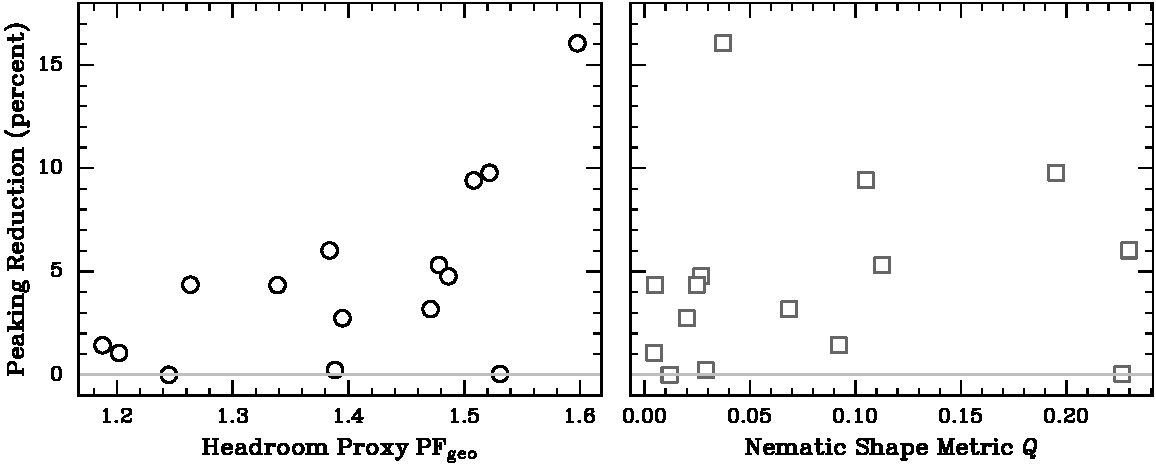
\includegraphics[width=0.77\linewidth]{predictor_scan.pdf}
  \note{The early small-sample correlation did not survive the fifteen-device test. PFgeo has a borderline Spearman coefficient of +0.525; Q is +0.396. These descriptors remain useful for geometry and feasibility, but neither closes the transport response.\notesources{Frozen data and exact rank statistics: \localpath{spf_prototype/paper/data/predictor_n15.csv}; interpretation: \localpath{spf_prototype/talk/QA_RESEARCH.md}.}}
\end{frame}

% 27
\begin{frame}{Returning to Neutronics-Informed Automatic Optimization}
  \centering
  \includegraphics[height=0.68\textheight]{/Users/tkiker/Downloads/Failure Slide Full Logo.jpg}
  \note{This is a deliberate visual break. The cheap geometric ranking did not answer the transport question, so the optimizer must retain OpenMC as the high-fidelity evaluator.\notesources{User-supplied image: \localpath{/Users/tkiker/Downloads/Failure Slide Full Logo.jpg}.}}
\end{frame}

% 28
\begin{frame}{Using ParaStell for Iterative Optimization}
  \begin{columns}[c,onlytextwidth]
    \begin{column}{0.52\textwidth}
      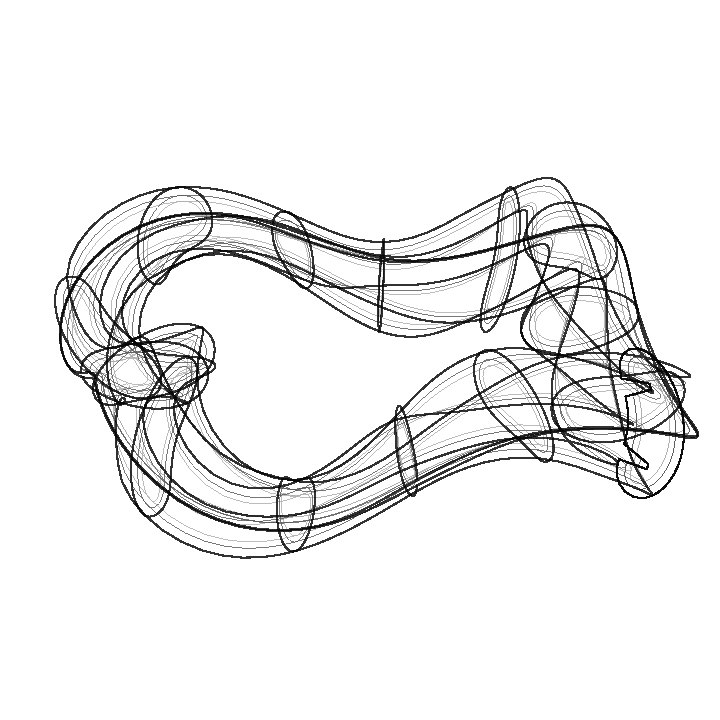
\includegraphics[width=0.94\linewidth]{parastell_iteration_bw.pdf}
    \end{column}
    \begin{column}{0.42\textwidth}
      ParaStell regenerates the nonuniform breeder and shield surfaces for each candidate.

      \vspace{0.24cm}
      Initial contrast
      \[
        \Delta t_{\mathrm{sh}}=-\Delta t_{\mathrm{br}}
      \]
      at a fixed outer envelope.

      \vspace{0.20cm}
      Current comparison: composition swap, added build, and clearance-constrained redistribution.
    \end{column}
  \end{columns}
  \note{The fixed-envelope breeder-for-shield trade was the first intervention family; the project is not assuming it is the only useful actuator. It can remove moderator while adding WC, so added-build and clearance-constrained contrasts are necessary. The wireframes show the actual QH plasma and two offset surfaces.\notesources{ParaStell interface and Step-1 builder: \localpath{spf_prototype/shield_opt/patch_worth/build_step1.py}; intervention records: \localpath{spf_prototype/shield_opt/patch_worth}.}}
\end{frame}

% 29
\begin{frame}[t]{Optimization Metric Selection (I/II)}
  \centering
  \vspace{0.04cm}
  \begin{columns}[T,totalwidth=0.94\textwidth]
    \begin{column}{0.30\textwidth}
      Attribution
      \slideline
      \begin{minipage}[t][1.10cm][t]{\linewidth}
        \vspace{0.26cm}
        \centering
        $\displaystyle A(\mathbf{x})=S(\mathbf{x})\psi^{\dagger}(\mathbf{x})$
      \end{minipage}
      \begin{minipage}[t][0.95cm][t]{\linewidth}
        \vspace{0.10cm}
        \raggedright
        Where harmful histories are born.
      \end{minipage}
      \begin{minipage}[t][0.70cm][t]{\linewidth}
        \vspace{0.22cm}
        {\fontsize{8.0}{9.4}\selectfont Domain: plasma}
      \end{minipage}
    \end{column}
    \begin{column}{0.30\textwidth}
      Worth
      \slideline
      \begin{minipage}[t][1.10cm][t]{\linewidth}
        \vspace{0.26cm}
        \centering
        $\displaystyle W_k=\int_{V_k}\phi\,\psi^{\dagger}\,\mathrm{d}V$
      \end{minipage}
      \begin{minipage}[t][0.95cm][t]{\linewidth}
        \vspace{0.10cm}
        \raggedright
        Where coil-important flux visits the existing build.
      \end{minipage}
      \begin{minipage}[t][0.70cm][t]{\linewidth}
        \vspace{0.22cm}
        {\fontsize{8.0}{9.4}\selectfont Domain: shield}
      \end{minipage}
    \end{column}
    \begin{column}{0.30\textwidth}
      Clearance
      \slideline
      \begin{minipage}[t][1.10cm][t]{\linewidth}
        \vspace{0.26cm}
        \centering
        $\displaystyle c(\vartheta,\phi)$
      \end{minipage}
      \begin{minipage}[t][0.95cm][t]{\linewidth}
        \vspace{0.10cm}
        \raggedright
        Where added material can physically fit.
      \end{minipage}
      \begin{minipage}[t][0.70cm][t]{\linewidth}
        \vspace{0.22cm}
        {\fontsize{8.0}{9.4}\selectfont Domain: winding-pack geometry}
      \end{minipage}
    \end{column}
  \end{columns}

  \vspace{0.46cm}
  \begin{minipage}{0.78\linewidth}
    \centering
    {\fontsize{8.8}{10.5}\selectfont Attribution cannot be back-projected directly into a shield-thickness update.}
  \end{minipage}
  \note{The initial idea was to compute source attribution in the plasma, project it onto the shield, and trade breeder thickness for more shield along that projection. The three columns show why that is incomplete: attribution, existing-build worth, and physical clearance answer different questions on different domains. The actual update requires a material-response derivative or a measured finite intervention.\notesources{Attribution and worth analysis: \localpath{spf_prototype/shield_opt/patch_worth}; status correction: \localpath{spf_prototype/shield_opt/patch_worth/analysis_bfd_20260824/analysis_status.md}.}}
\end{frame}

% 30
\begin{frame}[t]{Optimization Metric Selection (II/II)}
  \centering
  \vspace{0.08cm}
  \[
    \underset{\mathbf{u},\eta}{\operatorname{minimize}}\ \eta
    \qquad\text{subject to}\qquad
    R_j(\mathbf{u})\leq\eta\quad\text{for every coil }j
  \]

  \vspace{-0.02cm}
  \[
    \mathrm{TBR}(\mathbf{u})\geq \mathrm{TBR}_{\min},
    \qquad
    M_{\mathrm{sh}}(\mathbf{u})\leq M_{\max},
    \qquad
    t(\vartheta,\phi;\mathbf{u})\leq c(\vartheta,\phi)
  \]

  \vspace{0.16cm}
  \begin{minipage}{0.88\linewidth}
    {\fontsize{9.2}{11.1}\selectfont
    \raggedright
    Retain the complete response vector because reducing one coil can move the limiting response to another.

    \vspace{0.32cm}
    Compare equal-cost designs using peak magnet heating density, total cryogenic heating, and fast-neutron fluence.
    }
  \end{minipage}
  \note{The epigraph form makes the minimax objective explicit. The optimizer may use a smooth approximation internally, but every accepted design is judged against the actual complete coil-response vector. Equal-cost means exact shield mass, a TBR floor, and true winding-pack clearance rather than nominal cell counts or a circular-torus proxy.\notesources{Roadmap and metric requirements: \localpath{/Users/tkiker/Downloads/CLAUDE(20260824-005225).md}; optimizer scaffold: \localpath{spf_prototype/shield_opt/bayes_optimizer.py}.}}
\end{frame}

% 31
\begin{frame}{Choosing the Search Strategy}
  \begin{columns}[T,onlytextwidth]
    \begin{column}{0.46\textwidth}
      Gaussian-Process Bayesian Search
      \slideline
      $8$--$20$ smooth surface modes

      \vspace{0.17cm}
      Expected improvement under noisy, expensive OpenMC evaluations

      \vspace{0.17cm}
      Global exploration with explicit constraints
    \end{column}
    \begin{column}{0.46\textwidth}
      Empirical Response-Operator Update
      \slideline
      Finite interventions estimate $B_{\mathrm{FD}}$

      \vspace{0.17cm}
      A constrained minimax step selects the next candidate

      \vspace{0.17cm}
      Full OpenMC corrects nonlinearity after each step
    \end{column}
  \end{columns}

  \vspace{0.42cm}
  \centering
  Both strategies keep the transport calculation in the loop.
  \note{The repository contains a GP/expected-improvement scaffold. A second path uses the measured finite-intervention response matrix as a local operator, then re-evaluates in OpenMC. CMA-ES appeared in an early outline, but it is not the current strategy because direct fitting to Monte Carlo noise is poorly controlled.\notesources{Bayesian optimizer: \localpath{spf_prototype/shield_opt/bayes_optimizer.py}; roadmap and scope correction: \localpath{/Users/tkiker/Downloads/CLAUDE(20260824-005225).md}; early outline: \localpath{spf_prototype/talk/summer_recap_outline_2026-08-24.md}.}}
\end{frame}

% 32
\begin{frame}{Optimizing for Optimization}
  \centering
  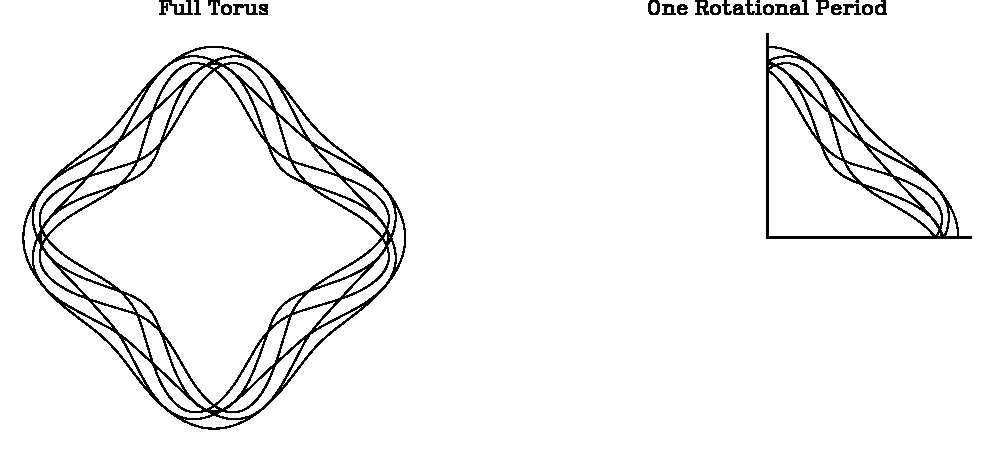
\includegraphics[width=0.69\linewidth]{periodic_boundaries_bw.pdf}

  \vspace{0.20cm}
  {\fontsize{8.8}{10.8}\selectfont
  \mbox{Rotationally periodic models keep histories that cross a field-period boundary (open wedges don't).}}
  \vspace{0.15cm}
  {\fontsize{8.8}{10.8}\selectfont Working on Surface Source Read (SSR) implementation currently.}
  \note{For the QH equilibrium, one rotational period is one quarter of the torus. The slide compares the full reference with the periodic candidate. The reduced model remains a computational hypothesis until it matches an identically normalized full-torus run. SSR remains active implementation work; the current effort must preserve field-period crossings and reproduce the complete coil-response vector before it can replace direct transport.\notesources{Periodic-boundary implementation: \localpath{spf_prototype/shield_opt/fwcadis/reciprocity_cadis/source_snapshot/build_oneperiod.py}; SSR work: \localpath{spf_prototype/shield_opt/patch_worth/build_step1.py}; status: \localpath{spf_prototype/shield_opt/patch_worth/analysis_bfd_20260824/analysis_status.md}.}}
\end{frame}

% 34
\begin{frame}{Early Optimization Caveats}
  \begin{columns}[c,onlytextwidth]
    \begin{column}{0.45\textwidth}
      \[
        \mathrm{FLiBe}\longrightarrow\mathrm{WC}
      \]
      \[
        \Delta t_{\mathrm{sh}}=-\Delta t_{\mathrm{br}}
      \]

      \vspace{0.20cm}
      More high-density shield is added while neutron moderation and breeding volume are removed.
    \end{column}
    \begin{column}{0.47\textwidth}
      The fast component can increase even when total attenuation improves.

      \vspace{0.10cm}
      Multiple scattering connects one material change to several coils.

      \vspace{0.26cm}
      Plasma attribution therefore cannot be projected directly onto a shield thickness update.
    \end{column}
  \end{columns}
  \note{The early fixed-envelope result was not a verdict on nonuniform shielding. It tested one coupled material swap. The current program separates composition swap, added build, and redistribution within clearance so the mechanism can be identified.\notesources{Fixed-envelope studies: \localpath{spf_prototype/shield_opt/patch_worth}; scope correction: \localpath{/Users/tkiker/Downloads/CLAUDE(20260824-005225).md}.}}
\end{frame}

% 35
\begin{frame}{Shielding Optimization: Current Status}
  \centering
  \vfill
  \begin{minipage}{0.90\linewidth}
    {\fontsize{9.2}{11.2}\selectfont End-to-End Design Loop Operational: ParaStell rebuilds nonuniform layers and OpenMC returns the complete coil-response vector with rotationally periodic transport.\par}

    \vspace{0.44cm}
    {\fontsize{9.2}{11.2}\selectfont Coarse Placement Sensitivity Resolved: A $12\times20$ intervention study identifies broad shield placements that reduce the limiting coil cluster---and others that increase loading.\par}

    \vspace{0.44cm}
    {\fontsize{9.2}{11.2}\selectfont Engineering Normalization Underway: Volume-normalized flux still peaks at coil 20; independent-seed reproduction, exact material mass, and clearance constraints are being finalized.\par}
  \end{minipage}
  \vfill
  \note{The end-to-end ParaStell-to-OpenMC loop is operational and returns the complete twenty-coil response vector. The coarse $12\times20$ intervention matrix establishes placement sensitivity, including both reducers and backfires. The remaining normalization gates are independent-seed reproduction, exact geometry-derived material mass, and winding-pack clearance.\notesources{Current correction and validation gates: \localpath{spf_prototype/shield_opt/patch_worth/analysis_bfd_20260824/analysis_status.md}; reconstructed vectors: \localpath{spf_prototype/shield_opt/patch_worth/analysis_bfd_20260824/patch_response_vectors.csv}.}}
\end{frame}

% 36
\begin{frame}{Next Steps for Optimization}
  \centering
  \vfill
  \begin{minipage}{0.90\linewidth}
    {\fontsize{9.2}{11.2}\selectfont Validate the Observed Control: Repeat the strongest interventions independently and evaluate magnet heating density, fast-neutron flux, TBR, and exact material cost.\par}

    \vspace{0.44cm}
    {\fontsize{9.2}{11.2}\selectfont Establish Spatial Convergence: Optimize successively finer, clearance-constrained design spaces until both performance and shield geometry stabilize.\par}

    \vspace{0.44cm}
    {\fontsize{9.2}{11.2}\selectfont Measure the Value of Response Awareness: Compare uniform, clearance-driven, wall-loading-driven, attribution-guided, and response-aware designs on equal-cost Pareto fronts.\par}
  \end{minipage}
  \vfill
  \note{The next phase has three gates. First, independently reproduce the strongest controls and score the complete engineering response. Second, refine the clearance-constrained spatial basis until the result is stable. Third, compare response-aware optimization with uniform and lower-information design rules on equal-cost Pareto fronts.\notesources{Locked roadmap: \localpath{/Users/tkiker/Downloads/CLAUDE(20260824-005225).md}; current gate status: \localpath{spf_prototype/shield_opt/patch_worth/analysis_bfd_20260824/analysis_status.md}.}}
\end{frame}

% 37
\begin{frame}{Summary}
  \begin{columns}[c,onlytextwidth]
    \begin{column}{0.47\textwidth}
      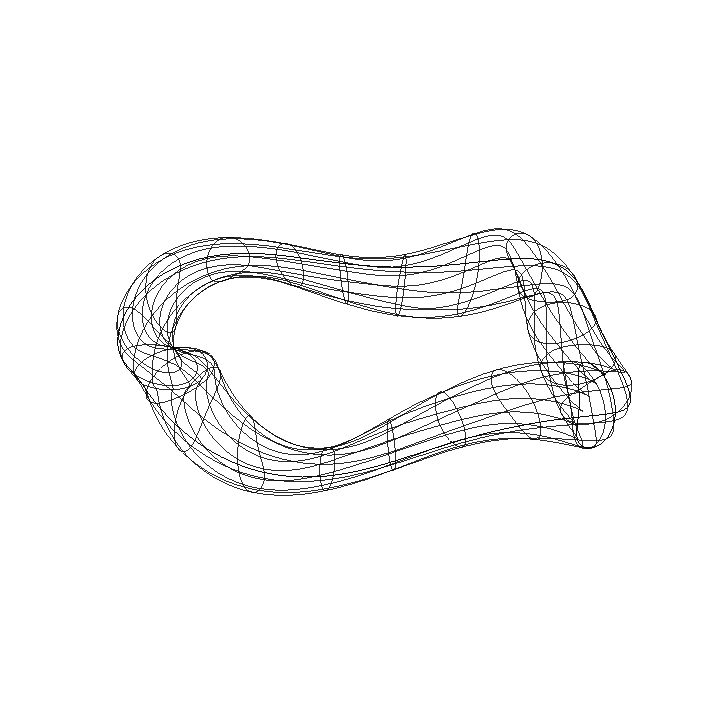
\includegraphics[width=0.92\linewidth]{title_stellarator_bw.pdf}
    \end{column}
    \begin{column}{0.46\textwidth}
      A VMEC-native OpenMC stellarator source with independent source-space and transport-space validation.

      \vspace{0.34cm}
      One spin-polarized emission kernel shared by tokamak and stellarator sources.

      \vspace{0.34cm}
      A transport-in-loop shielding framework that now resolves placement sensitivity and has a defined path to an equal-cost constrained optimum.
    \end{column}
  \end{columns}
  \note{Close at the actual maturity level. The source and SPF work are mature method contributions. The shielding framework is operational, but the equal-cost optimization and full-fidelity validation remain future work.\notesources{Project evidence: \localpath{spf_prototype/native_spf}; \localpath{spf_prototype/paper}; \localpath{spf_prototype/shield_opt}.}}
\end{frame}

\appendix

{\setbeamertemplate{footline}{}
\begin{frame}[plain,noframenumbering]
  \vfill
  {\fontsize{12}{14}\selectfont IV\par}
  \vspace{0.38cm}
  {\fontsize{22}{27}\selectfont Backup Slides\par}
  \vfill
\end{frame}}

\begin{frame}{Tokamak Local-Field Model}
  \centering
  \[
    \Bhat=
    \frac{\widehat{\boldsymbol\phi}+s\lambda\widehat{\mathbf p}}
    {\left\lVert\widehat{\boldsymbol\phi}+s\lambda\widehat{\mathbf p}\right\rVert},
    \qquad
    \lambda=\frac{r}{q(\rho)R},
    \qquad
    \rho=\frac{r}{a}.
  \]

  \vspace{0.10cm}
  \begin{columns}[T,onlytextwidth]
    \begin{column}{0.44\textwidth}
      {\fontsize{8.8}{10.6}\selectfont
      $r$: Miller flux-surface minor-radius label at the sampled birth point.

      \vspace{0.10cm}
      $a$: edge minor radius; $\rho$ is the normalized radius.

      \vspace{0.18cm}
      $R$: local cylindrical major radius, measured from the tokamak symmetry axis.
      }
    \end{column}
    \begin{column}{0.48\textwidth}
      {\fontsize{8.8}{10.6}\selectfont
      $q(\rho)$: safety factor, the toroidal turns of a field line per poloidal turn.

      \vspace{0.18cm}
      $\lambda$: local poloidal-to-toroidal field ratio, approximately $B_p/B_\phi$.

      \vspace{0.18cm}
      $\widehat{\mathbf p}$: unit poloidal tangent; $\widehat{\boldsymbol\phi}$: toroidal unit vector; $s=\pm1$: field handedness.
      }
    \end{column}
  \end{columns}

  \vspace{0.27cm}
  {\fontsize{9.0}{10.8}\selectfont This approximation is used only by \texttt{TokamakSource}; \texttt{StellaratorSource} interpolates the cylindrical field components $(B_R,B_\phi,B_Z)$ from VMEC.}
  \note{Peterson's Miller source supplies $r$, $a$, $R$, and the poloidal surface tangent at each sampled birth point. The safety factor fixes the field-line pitch through the cylindrical relation $B_p/B_\phi\approx r/(qR)$. The handedness sign selects the direction of the poloidal component. In the limit $q\rightarrow\infty$, the field becomes purely toroidal. The stellarator source does not use this approximation; it interpolates the equilibrium field components and normalizes them.\notesources{Tokamak field model: \localpath{spf_prototype/native_spf/source.cpp}. Stellarator field model: \localpath{spf_prototype/native_spf/stellarator_source.cpp}.}}
\end{frame}

\begin{frame}{\texttt{StellaratorSource}: Computational Notes}
  \centering
  {\fontsize{8.8}{10.6}\selectfont
  \texttt{read\_fluxmap()} $\longrightarrow$ \texttt{build\_cdf\_cascade()} $\longrightarrow$ \texttt{sample(seed)} $\longrightarrow$ \texttt{SourceSite}}

  \vspace{0.02cm}
  {\fontsize{8.4}{10.0}\selectfont Read-only state makes \texttt{sample()} thread-safe; position sampling is rejection free with unit weight.}

  \vspace{0.05cm}
  \begin{columns}[T,onlytextwidth]
    \begin{column}{0.46\textwidth}
      Initialization
      \slideline
      {\fontsize{8.6}{10.3}\selectfont
      \texttt{spf\_fluxmap\_v1} loads a text \texttt{.meta} header and little-endian \texttt{.bin} arrays for $(\rho,\vartheta,\zeta)$, $\sqrt g$, geometry, and cylindrical $\mathbf B$.

      \vspace{0.10cm}
      The constructor forms $S(\rho)\lvert\sqrt g\rvert$ and stores three normalized CDF tables: \texttt{cdf\_rho\_}, \texttt{cdf\_zeta\_}, and \texttt{cdf\_theta\_}.

      \vspace{0.10cm}
      Python writes XML; \texttt{polarization=None} omits SPF elements and retains the isotropic fallback.
      }
    \end{column}
    \begin{column}{0.46\textwidth}
      Each Sample Call
      \slideline
      {\fontsize{8.6}{10.3}\selectfont
      \texttt{upper\_bound\_strided()} selects a cell in the order $\rho\rightarrow\zeta\rightarrow\vartheta$; three additional pseudorandom numbers jitter within it.

      \vspace{0.10cm}
      \texttt{interp()} performs trilinear interpolation: $\rho$ is clamped, while $\vartheta$ and $\zeta$ wrap periodically.

      \vspace{0.10cm}
      Interpolated geometry gives the Cartesian birth site; interpolated $(B_R,B_\phi,B_Z)$ gives $\Bhat$. Angle, energy, and time are then sampled.
      }
    \end{column}
  \end{columns}

  \note{The implementation is split deliberately between a portable equilibrium file, a Python API/XML layer, and the native C++ sampler. The binary payload is fixed-order C-contiguous double precision. The CDF cascade is constructed once, not rebuilt per history. At sample time all lookup tables are read-only, which avoids shared mutable state under OpenMP. The C++ index convention and interpolation order reproduce the independent NumPy mirror.\notesources{C++ interface and invariants: \localpath{spf_prototype/native_spf/stellarator_source.h}. Native implementation: \localpath{spf_prototype/native_spf/stellarator_source.cpp}. Python API: \localpath{spf_prototype/native_spf/stellarator_source.py}. Flux-map writer: \localpath{spf_prototype/python/quasr_fluxmap.py}.}}
\end{frame}

\begin{frame}{SPF Emission Kernel: Symbol Reference}
  \centering
  \[
    \eta=a+\frac{2}{3}b+\frac{1}{3}c,
    \qquad
    \frac{R_f}{R_{f,0}}=\frac{3}{2}\eta,
    \qquad
    P_\perp=\frac{a}{\eta},
    \qquad
    x=\uhat\cdot\Bhat=\cos\theta.
  \]

  \vspace{0.00cm}
  \begin{columns}[T,onlytextwidth]
    \begin{column}{0.46\textwidth}
      {\fontsize{8.8}{10.6}\selectfont
      $a$: same-sign D--T spin projections; $b$: zero deuteron spin projection, $m_D=0$; $c$: opposite-sign projections. The populations satisfy $a+b+c=1$.

      \vspace{0.10cm}
      $\eta$: total-rate coefficient; $R_f/R_{f,0}$ is the fusion-rate multiplier relative to unpolarized fuel.

      \vspace{0.10cm}
      $P_\perp$: probability of selecting the perpendicular angular kernel.
      }
    \end{column}
    \begin{column}{0.46\textwidth}
      {\fontsize{8.8}{10.6}\selectfont
      $\uhat$: sampled neutron birth direction; $\Bhat$: local magnetic-field direction; $x$: pitch cosine relative to the field.
      \[
        p_\perp(x)=\frac{3}{4}(1-x^2),
        \qquad
        p_\parallel(x)=\frac{1}{4}+\frac{3}{4}x^2.
      \]
      A mode $(1,0,0)$ gives $1.5$ times the unpolarized rate and perpendicular emission. B and C use the parallel kernel.
      }
    \end{column}
  \end{columns}
  \note{The state populations determine two separate outputs: the total reaction-rate multiplier and the angular mixture. Unpolarized fuel has $a=b=c=1/3$, so $\eta=2/3$, $R_f/R_{f,0}=1$, $P_\perp=1/2$, and the combined pitch-cosine distribution is flat. Pure A gives a rate multiplier of 1.5 and the perpendicular kernel. Pure B retains the unpolarized rate; pure C halves it. B and C nevertheless share the same parallel angular shape.\notesources{Kernel derivation and implementation: \localpath{spf_prototype/native_spf/source.cpp}; tests: \localpath{spf_prototype/native_spf/test_spf_tokamak.py}.}}
\end{frame}

\begin{frame}{SPF Kernel: Computational Notes}
  \centering
  {\fontsize{8.8}{10.6}\selectfont
  \texttt{polarization} $\longrightarrow p_\perp$ $\longrightarrow \cos\theta$ $\longrightarrow \widehat{\mathbf u}_{\rm local}$ $\longrightarrow \widehat{\mathbf u}_{\rm global}$}

  \vspace{0.02cm}
  {\fontsize{8.4}{10.0}\selectfont Per-neutron sampler: \texttt{SourceSite::wgt} is unchanged; absolute rate uses source strength or postprocessing.}

  \vspace{0.05cm}
  \begin{columns}[T,onlytextwidth]
    \begin{column}{0.46\textwidth}
      Initialization
      \slideline
      {\fontsize{8.6}{10.3}\selectfont
      XML $(a,b,c)$ is validated and normalized; the constructor stores $p_\perp=a/\eta$. If absent, the original isotropic path is used.

      \vspace{0.10cm}
      Field direction: \texttt{TokamakSource} uses \texttt{toroidal} or $q$-profile \texttt{pitched}; \texttt{StellaratorSource} uses \texttt{fluxmap} or a toroidal cross-check.

      \vspace{0.10cm}
      Both sources call the same \texttt{sample\_polarized\_direction()} routine.
      }
    \end{column}
    \begin{column}{0.46\textwidth}
      Each Direction Draw
      \slideline
      {\fontsize{8.6}{10.3}\selectfont
      Fixed PRNG order: mode selector, inverse-CDF uniform variate, then local azimuth. This enables fixed-seed parity tests.

      \vspace{0.10cm}
      The perpendicular and parallel $\cos\theta$ laws use exact cubic inverse CDFs, eliminating angular rejection loops.

      \vspace{0.10cm}
      Least-aligned-axis Gram--Schmidt avoids parallel-axis degeneracy before global rotation.
      }
    \end{column}
  \end{columns}

  \note{This slide describes the actual native path rather than the physics derivation. The constructor converts mode populations to a normalized shape-selection probability. Each call consumes three angular random numbers in a fixed order, solves the analytic inverse CDF for pitch cosine, chooses a uniform azimuth, and rotates the local vector into global coordinates. The least-aligned-axis construction makes the frame stable for any field orientation. Tests cover the isotropic limit, pure modes, rotation, field models, validation failures, and Python/XML round trips. The implementation intentionally keeps the angular sampler normalized per source neutron; the separate total-rate factor eta was restored in absolute-rate studies by source normalization or postprocessing.\notesources{Native tokamak implementation: \localpath{spf_prototype/native_spf/source.cpp}. Stellarator reuse: \localpath{spf_prototype/native_spf/stellarator_source.cpp}. Python and XML tests: \localpath{spf_prototype/native_spf/test_spf_tokamak.py}. Absolute-rate treatment: \localpath{spf_prototype/python/tier7_absolute.py}.}}
\end{frame}

\begin{frame}{Adjoint Computation}
  \centering
  {\fontsize{8.7}{10.5}\selectfont
  \[
    L^\dagger\psi_j^\dagger=q_j,
    \qquad
    A_j(\mathbf r)=\int S(\mathbf r,E,\Omega)\,\psi_j^\dagger(\mathbf r,E,\Omega)\,\mathrm dE\,\mathrm d\Omega,
    \qquad
    R_j=\int A_j(\mathbf r)\,\mathrm dV.
  \]}

  \vspace{0.02cm}
  \begin{columns}[T,onlytextwidth]
    \begin{column}{0.46\textwidth}
      {\fontsize{8.7}{10.5}\selectfont
      $L^\dagger$: adjoint transport operator; it propagates response importance backward through the reactor.

      \vspace{0.10cm}
      $q_j$: coil-$j$ response source: fast flux or copper kerma (energy transferred per mass).

      \vspace{0.10cm}
      $\psi_j^\dagger$: importance of a neutron state $(\mathbf r,E,\Omega)$: position, energy, and direction.

      \vspace{0.10cm}
      Scope: one adjoint gives attribution for one response, not a shield-material derivative.
      }
    \end{column}
    \begin{column}{0.46\textwidth}
      {\fontsize{8.7}{10.5}\selectfont
      $S$: plasma birth source; $A_j$: where histories responsible for response $j$ are born; $R_j$: scalar coil response.

      \vspace{0.10cm}
      OpenMC method: multigroup random ray (deterministic track-based transport) with a filamentary adjoint source along the target coil.

      \vspace{0.10cm}
      Reciprocity: $\int S\psi_j^\dagger$ reproduced the forward coil ranking (Spearman rank $0.76$ for QH; $0.83$ for QA).
      }
    \end{column}
  \end{columns}

  \note{This is the attribution calculation actually used. A localized adjoint source was sampled along a target coil filament and given either flat fast-energy weighting or a copper-kerma response spectrum. OpenMC's multigroup random-ray adjoint solve returns the importance field. Multiplying by the physical source gives the contributon or source-attribution density. Reciprocity then compares its integral with a separate forward per-coil tally. One adjoint corresponds to one scalar response: changing the target coil or changing from fast flux to heating requires a new response source.\notesources{Adjoint implementation: \localpath{spf_prototype/shield_opt/fwcadis/adjoint_importance.py}. Reciprocity calculation: \localpath{spf_prototype/shield_opt/fwcadis/reciprocity_check.py}. Reported validation: \localpath{spf_prototype/talk/peterson_checkin_2026-07-27.tex}.}}
\end{frame}

\begin{frame}{FW-CADIS and Weight Windows}
  \centering
  {\fontsize{9.0}{10.8}\selectfont Forward-Weighted Consistent Adjoint-Driven Importance Sampling}

  \vspace{-0.10cm}
  \[
    \text{forward random-ray flux }\psi
    \longrightarrow
    \text{adjoint importance }\psi^\dagger
    \longrightarrow
    \text{weight windows }(w_L,w_U).
  \]

  \vspace{-0.10cm}
  \begin{minipage}{0.91\linewidth}
    \raggedright
    {\fontsize{8.7}{10.4}\selectfont
    $w_L,w_U$: particle-weight bounds. Histories above $w_U$ split; those below $w_L$ undergo Russian roulette. Correct accounting preserves the expected tally while moving effort to important phase space.

    \vspace{0.10cm}
    What Ran: A one-period DAGMC (CAD-based geometry) pilot produced a $10\times10\times10$ map. Forward and adjoint source-region miss rates were $19.38\%$ and $43.39\%$: an integration result, not a production map.

    \vspace{0.10cm}
    What Was Used: The $12\times20$ matrix used analog forward transport without weight windows. The direct adjoint supplied attribution separately.
    }
  \end{minipage}
  \note{FW-CADIS and the direct adjoint share the adjoint-importance idea but produce different deliverables. The direct solve produces an importance field for attribution. FW-CADIS performs forward and adjoint random-ray calculations to generate weight-window bounds for a later Monte Carlo run. The native pilot successfully exercised OpenMC's machinery, but the coarse mesh and source-region miss rates made the windows unsuitable for scoring. In the SSR benchmark, the native map over-split, the continuous-energy reciprocity-CADIS approximation was effectively neutral, and the MAGIC map remained statistically unresolved. Therefore none was used in the clean finite-intervention result.\notesources{FW-CADIS plan: \localpath{spf_prototype/shield_opt/fwcadis/FWCADIS_PLAN.md}. Pilot results: \localpath{spf_prototype/shield_opt/fwcadis/RUN_RESULTS_2026-08-22.md}. SSR benchmark: \localpath{spf_prototype/shield_opt/fwcadis/ssr_benchmark/RUN_RESULTS_2026-08-22.md}. Analog intervention audit: \localpath{spf_prototype/shield_opt/patch_worth/analysis_bfd_20260824/analysis_status.md}.}}
\end{frame}

\begin{frame}{Surface Source Read (SSR)}
  \begin{columns}[T,onlytextwidth]
    \begin{column}{0.44\textwidth}
      Method
      \slideline
      {\fontsize{8.8}{10.6}\selectfont
      Write: bank each particle crossing a selected surface, including position $\mathbf r$, direction $\uhat$, energy $E$, statistical weight $w$, and time $t$.

      \vspace{0.15cm}
      Read: relaunch that bank through a changed downstream geometry instead of resampling the plasma.

      \vspace{0.15cm}
      Exactness requires a clean separation between unchanged upstream transport and the varied downstream problem, without lost or double-counted crossings.
      }
    \end{column}
    \begin{column}{0.48\textwidth}
      First-Wall Test
      \slideline
      {\fontsize{8.8}{10.6}\selectfont
      A first-wall bank kept breeder and shield downstream and therefore editable.

      \vspace{0.15cm}
      The nonconvex torus produced $2.36$ records per birth; $58\%$ were scattered recrossings. Fresh-history filtering recovered the inboard response to $4.1\%$ CV (coefficient of variation).

      \vspace{0.15cm}
      Far coils remained $3.5$--$5$ times low; replay saved only $11$--$13\%$ because blanket and shield scattering still ran.

      \vspace{0.15cm}
      Status: not used for the current intervention matrix.
      }
    \end{column}
  \end{columns}

  \note{SSR means surface-source write and read. The intended use was to run plasma-to-first-wall transport once and replay the same bank through many breeder and shield candidates. The toroidal first wall is nonconvex, so particles can scatter in the blanket, cross back through the plasma void, and cross the recording surface again. Replaying every record double-counted those histories. Filtering to uncollided 14.06 MeV births fixed the peak-load region but did not reproduce indirect paths to far coils. A benign normalization error was also corrected, but the far-coil deficit remained systematic. Freezing deeper would reduce work and avoid some recrossing problems, but it would also bake part or all of the variable radial build into the bank.\notesources{SSR diagnosis and timings: \localpath{spf_prototype/talk/granola_context_2026-08-19.md}; teaching notes: \localpath{spf_prototype/talk/peterson_checkin_2026-08-19_notes.tex}; controlled variance-reduction benchmark: \localpath{spf_prototype/shield_opt/fwcadis/ssr_benchmark/RUN_RESULTS_2026-08-22.md}.}}
\end{frame}

\begin{frame}{Alpha Self-Heating Beyond the Cross-Section Gain}
  \centering
  \vspace{-0.08cm}
  \[
    D+T\longrightarrow \alpha\,(3.5\ \mathrm{MeV})+n\,(14.1\ \mathrm{MeV}),
    \qquad
    P_\alpha=\frac{3.5}{17.6}P_f\approx0.20P_f
  \]

  \vspace{-0.04cm}
  \[
    \sigma_{DT}\uparrow
    \ \Longrightarrow\ 
    P_f\uparrow
    \ \Longrightarrow\ 
    P_\alpha\uparrow
    \ \Longrightarrow\ 
    T_i\uparrow
    \ \Longrightarrow\ 
    \langle\sigma v\rangle\uparrow
  \]

  \vspace{0.04cm}
  \begin{minipage}{0.90\linewidth}
    {\fontsize{8.8}{10.5}\selectfont
    The A-state $\sin^2\theta$ kernel biases alpha birth velocity perpendicular to $\Bhat$, but more $v_\perp$ does not make the gyro-orbit tighter:
    \[
      r_{L\alpha}=\frac{m_\alpha v_\perp}{2eB}.
    \]
    Anisotropic-alpha confinement requires a fast-ion orbit calculation. The established greater-than-$50\%$ power gain is the nonlinear self-heating feedback above.
    }
  \end{minipage}
  \note{At fixed plasma state, a 50 percent reaction-rate increase gives 50 percent more alpha heating. In a burning plasma, however, that added heating changes the plasma state: ion temperature rises, the Maxwellian reactivity rises, and the burn can amplify further. The precise gain depends on transport and power balance, so do not quote one universal multiplier. Also correct the tempting gyro-orbit argument: for fixed energy, more perpendicular velocity means a larger Larmor radius. Whether the changed pitch distribution improves alpha retention is device dependent.\notesources{Heidbrink et al., Frontiers in Physics 12, 1355212 (2024), reactor-considerations section; Kulsrud et al., Physical Review Letters 49, 1248 (1982).}}
\end{frame}

\begin{frame}{Preparing and Losing Nuclear-Spin Polarization}
  \begin{columns}[T,onlytextwidth]
    \begin{column}{0.46\textwidth}
      {\fontsize{8.55}{10.25}\selectfont
      Prepare and Deliver
      \slideline
      Deuterium: Dynamic nuclear polarization in cryogenic LiD transfers electron order to deuterons; demonstrated vector polarization reaches about $70\%$.

      \vspace{0.15cm}
      $^3$He: Spin-exchange optical pumping precedes shell permeation; reported polarization reaches about $65\%$.

      \vspace{0.15cm}
      Delivery: Cryogenic injection and a continuous guide field preserve the axis. A polarized neutral beam is the principal alternative.
      }
    \end{column}
    \begin{column}{0.46\textwidth}
      {\fontsize{8.55}{10.25}\selectfont
      Depolarize
      \slideline
      Field Nulls: With no field, the reference axis is lost; injection therefore requires a guide field.

      \vspace{0.15cm}
      Bound Electrons and Surfaces: Hyperfine coupling during ionization, ablation, or recycling can scramble nuclear spin.

      \vspace{0.15cm}
      Resonant Fields: Waves near the nuclear precession frequency can drive spin flips. Core Coulomb collisions and nonresonant turbulence are predicted to be weak.
      }
    \end{column}
  \end{columns}
  \note{Dynamic nuclear polarization first polarizes electrons in a strong field at low temperature and then uses microwaves to transfer that order to deuterons. Helium-3 is polarized by spin-exchange optical pumping and loaded into a shell. Once the material is ionized, the main theoretical concern is a resonant electromagnetic perturbation near the nuclear Larmor frequency; Coulomb collisions do not efficiently flip nuclear spin. The injection and ablation phases are experimentally important because field gradients, partial ionization, bound-electron hyperfine coupling, and surface contact can depolarize the fuel before it reaches the core.\notesources{Heidbrink et al., Frontiers in Physics 12, 1355212 (2024), sections 3--5; Baylor et al., Nuclear Fusion 63, 076009 (2023).}}
\end{frame}

\begin{frame}{The DIII-D Program Will Measure Polarization Survival}
  \centering
  \[
    D+{}^3\mathrm{He}\longrightarrow
    \alpha\,(3.6\ \mathrm{MeV})+p\,(14.7\ \mathrm{MeV})
  \]

  \vspace{0.08cm}
  \begin{minipage}{0.91\linewidth}
    {\fontsize{9.15}{11.1}\selectfont
    Prepare the Proxy Fuel: Polarized LiD and $^3$He pellets reproduce the low-energy D--T spin physics without handling tritium.

    \vspace{0.34cm}
    Infer the Lifetime: The poloidal and pitch distributions of escaping protons and alphas retain information about the reactants' polarization state.

    \vspace{0.34cm}
    Program Status: By the 2025 APS-DPP update, Jefferson Lab had commissioned the LiD irradiation beamline while UVA, ORNL, and UCI were developing $^3$He pellets, cryogenic injection, plasma scenarios, and charged-product diagnostics. No polarization-lifetime result had yet been reported.
    }
  \end{minipage}
  \note{The D--3He reaction is an isospin-mirror proxy for D--T at fusion energies, so it tests the relevant spin dependence without tritium. DIII-D can infer the surviving polarization from relative charged-fusion-product distributions: 14.7 MeV protons preserve useful pitch information, while the wall strike pattern of 3.6 MeV alphas carries birth-angle information. The 2025 status report described active component development, not a completed lifetime measurement.\notesources{Heidbrink et al., Frontiers in Physics 12, 1355212 (2024); Garcia, Heidbrink, and Sandorfi, Nuclear Fusion 63, 026030 (2023); W. W. Heidbrink, Overview and Status of the Spin Polarized Fusion Program, APS-DPP 2025 oral abstract.}}
\end{frame}

\end{document}
